\chapter{Results and discussion}
\label{chap:results}

This chapter presents what the tool produced and how far its results can be
trusted. It starts with the verification results, because the case studies
depend on them. It then gives the three case studies, each with its designs,
checks, finite element results and parameter sweeps. The later sections show
the calculation package and the application, report run times, compare the
two phases of the project and answer the research questions. All numbers come
from the runs kept in \code{data/} with this report.

\section{Verification results}
\label{sec:verification-results}

The full benchmark suite ran in 27.9~s and every comparison passed its
tolerance. Table~\ref{tab:verification} lists the results and
Figure~\ref{fig:verification} plots each error against its tolerance on a log
scale.

\begin{table}[H]
\centering
\caption{Verification results}
\label{tab:verification}
\small
\begin{tabularx}{\textwidth}{>{\raggedright\arraybackslash}Xrrrr}
\toprule
\textbf{Quantity} & \textbf{Reference} & \textbf{\NEMO{}} & \textbf{Error} & \textbf{Tolerance}\\
\midrule
\multicolumn{5}{l}{\emph{Padeye hand calculation, 4~t on two points at 60$^\circ$, S355, 20~mm plate}}\\
Sling force $F$ (N) & 22,647.6 & 22,647.5 & $-0.0005\%$ & 0.1\%\\
Strength reduction $C_r$ & 0.885696 & 0.885696 & $0.0000\%$ & 0.1\%\\
Effective width $b_\text{eff}$ (mm) & 22.0013 & 22.0013 & $+0.0002\%$ & 0.1\%\\
Tension through pinhole $P_t$ (N) & 101,763 & 101,763 & $-0.0002\%$ & 0.1\%\\
Fracture beyond pinhole $P_b$ (N) & 117,933 & 117,933 & $0.0000\%$ & 0.1\%\\
Shear plane area $A_v$ (mm$^2$) & 1,492.61 & 1,492.61 & $+0.0003\%$ & 0.1\%\\
Double plane shear $P_v$ (N) & 136,408 & 136,408 & $+0.0003\%$ & 0.1\%\\
Pin bearing $P_p$ (N) & 54,912.5 & 54,912.5 & $0.0000\%$ & 0.1\%\\
Base combined use & 0.14898 & 0.148982 & $+0.0016\%$ & 0.1\%\\
Base weld stress (MPa) & 26.179 & 26.1788 & $-0.0008\%$ & 0.1\%\\
Plate mass (kg) & 2.5958 & 2.59578 & $-0.0006\%$ & 0.1\%\\
\midrule
\multicolumn{5}{l}{\emph{CAD volume against the exact formula}}\\
Plain padeye (mm$^3$) & 330,673 & 330,673 & $0.0000\%$ & 0.01\%\\
Padeye with cheek plates (mm$^3$) & 424,000 & 424,000 & $0.0000\%$ & 0.01\%\\
Pipe support bracket (mm$^3$) & 324,921 & 324,921 & $0.0000\%$ & 0.01\%\\
\midrule
\multicolumn{5}{l}{\emph{Cantilever, 3,487 elements, 19,479 equations}}\\
Tip deflection (mm) & 0.95981 & 0.95216 & $-0.80\%$ & 3\%\\
Bending stress at mid-span (MPa) & 75.0 & 76.97 & $+2.63\%$ & 4\%\\
\midrule
\multicolumn{5}{l}{\emph{Plate with a hole, 16,749 elements, 96,000 equations}}\\
Stress concentration factor & 3.0322 & 3.0597 & $+0.91\%$ & 5\%\\
\midrule
\multicolumn{5}{l}{\emph{Panel method}}\\
Lowest $C_p$ on a circle & $-3.000$ & $-2.998$ & $-0.05\%$ & 0.5\%\\
NACA 0012 lift slope (per rad) & 6.864 & 6.939 & $+1.09\%$ & 3\%\\
NACA 0020 lift slope (per rad) & 7.251 & 7.370 & $+1.65\%$ & 3\%\\
\midrule
\multicolumn{5}{l}{\emph{Fin stock, 6,160 elements, 31,584 equations}}\\
Equivalent stress near the bearing (MPa) & 165.67 & 165.46 & $-0.13\%$ & 4\%\\
\midrule
Support reactions, all three finite element models & & & $0.0000\%$ & $10^{-6}\%$\\
\bottomrule
\end{tabularx}
\end{table}

\begin{figure}[H]
\centering
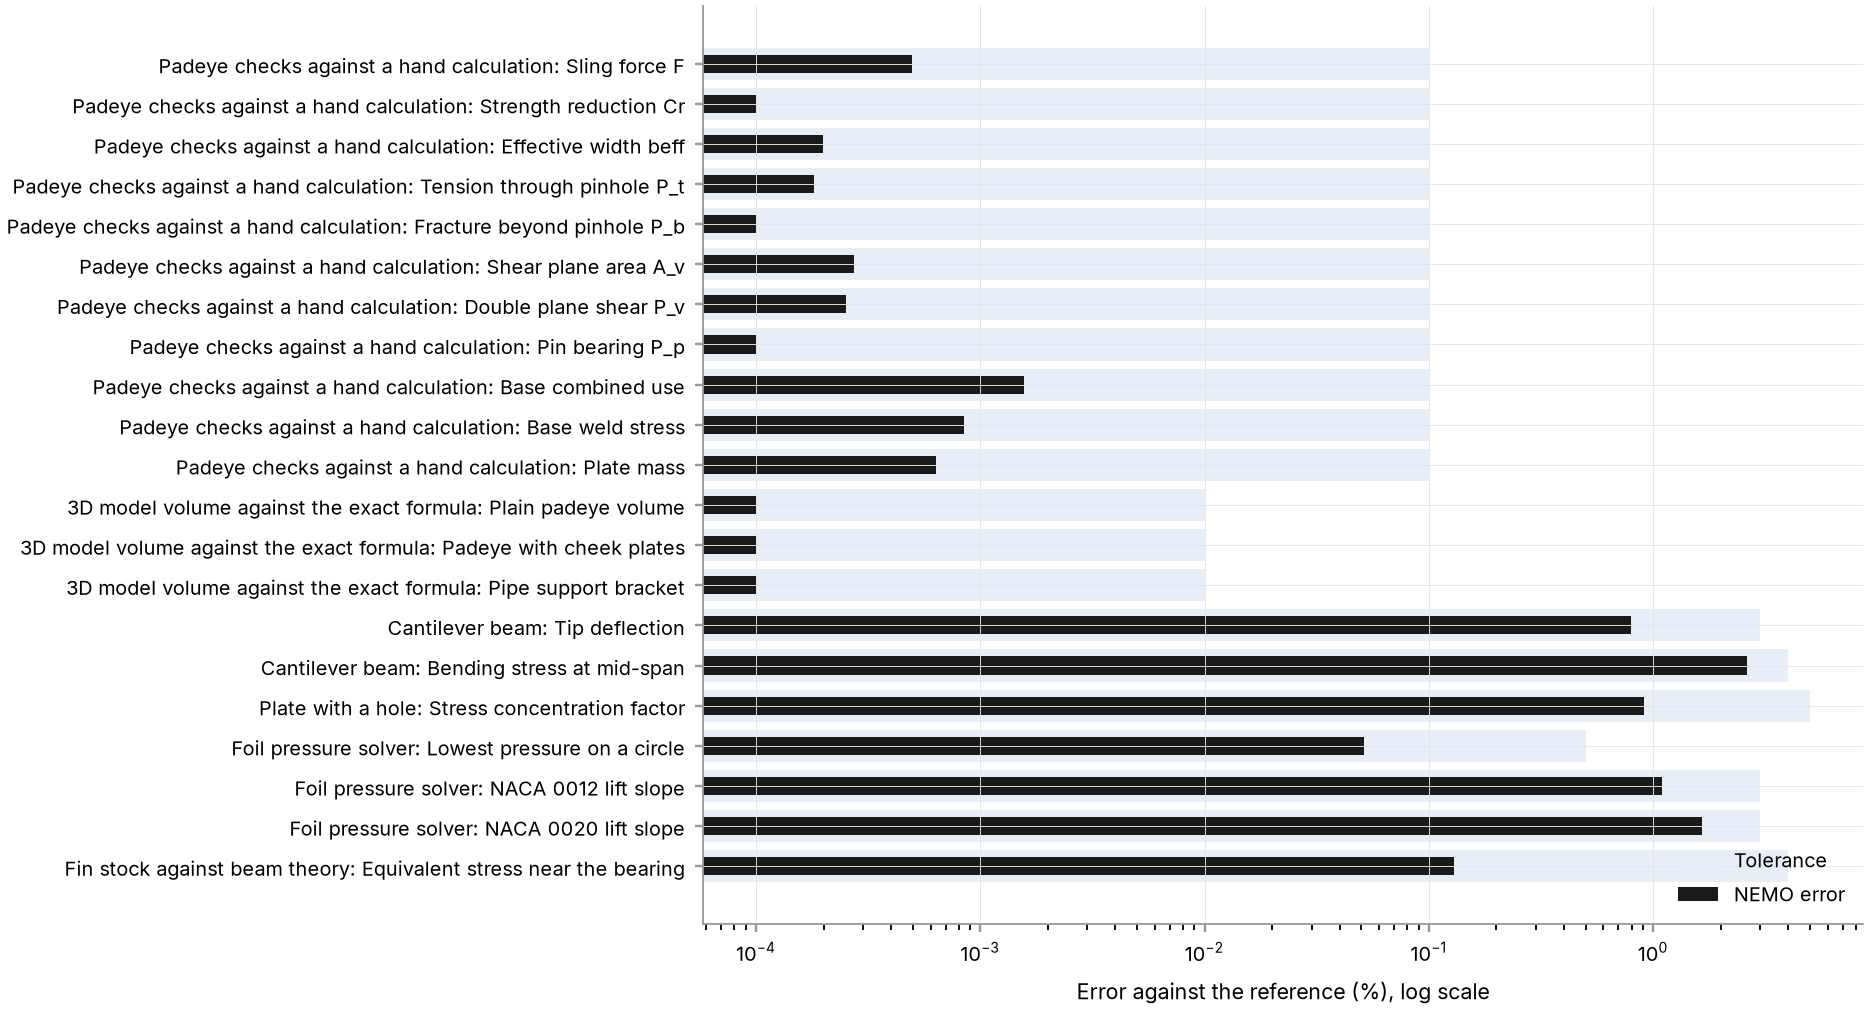
\includegraphics[width=0.95\textwidth]{images/verification.png}
\caption{Error of each verification quantity against its tolerance}
\label{fig:verification}
\end{figure}

The padeye hand calculation agrees to better than 0.002\% in every quantity.
The remaining differences come from rounding in the hand calculation, which
was carried to six significant figures. This confirms that the code
implements the BTH-1 expressions as written in the engineering manual. It
does not confirm that the manual reads BTH-1 correctly. That needs a published
worked example, which has not yet been done.

The CAD volumes match the formulas exactly. The geometry code and the mass
code were written separately, one from the build123d solid and one from the
analytic outline, so this agreement checks both.

The finite element errors are small and have the expected signs. The
cantilever tip deflection is 0.8\% low, which is consistent with the slight
stiffness of a coarse quadratic mesh. The mid-span bending stress is 2.6\%
high, inside its 4\% tolerance. The finite element value is a von Mises
stress averaged at mesh vertices, while beam theory gives the axial stress
alone. The two are not quite the same quantity, and a difference of a few per
cent is expected at this mesh density. The stress concentration factor of the
plate with a hole is
0.9\% above Heywood's value \cite{peterson2008}. The fin stock agrees with beam
and torsion theory to 0.13\%.

Figure~\ref{fig:panel-validation} shows the panel method results. On a
circle, where the exact pressure is $C_p = 1 - 4\sin^2\theta$, the 160-panel
solution is indistinguishable from the exact curve. The section lift slopes
lie 1\% to 2\% above the thick-section estimate $2\pi(1 + 0.77t/c)$
\cite{abbott1959}. That estimate is itself an approximation and an inviscid
method is expected to sit slightly high, so this is a reasonable result.
Measured slopes for real sections are lower again because of the boundary
layer, which is one reason the fin load does not use the panel method for its
force.

\begin{figure}[H]
\centering
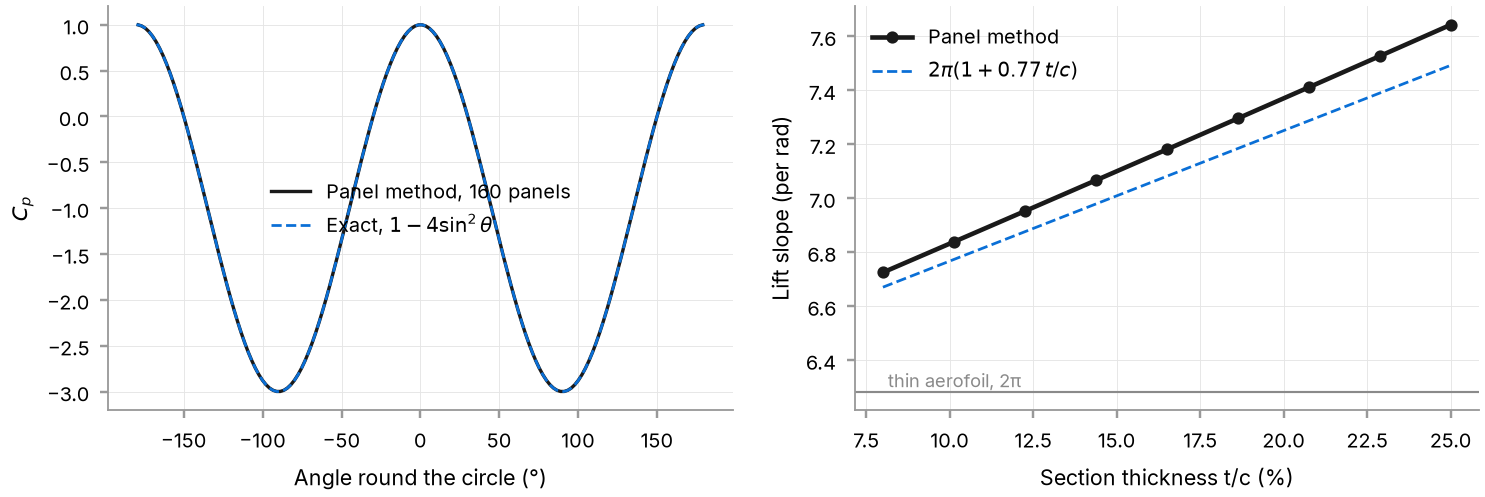
\includegraphics[width=0.95\textwidth]{images/panel-validation.png}
\caption{Panel method against the exact flow round a circle and the
thick-section lift slope}
\label{fig:panel-validation}
\end{figure}

All 153 automated tests passed on the final version of the engine. The
benchmarks can also be run from the application (Figure~\ref{fig:app-verification}).

\begin{figure}[H]
\centering
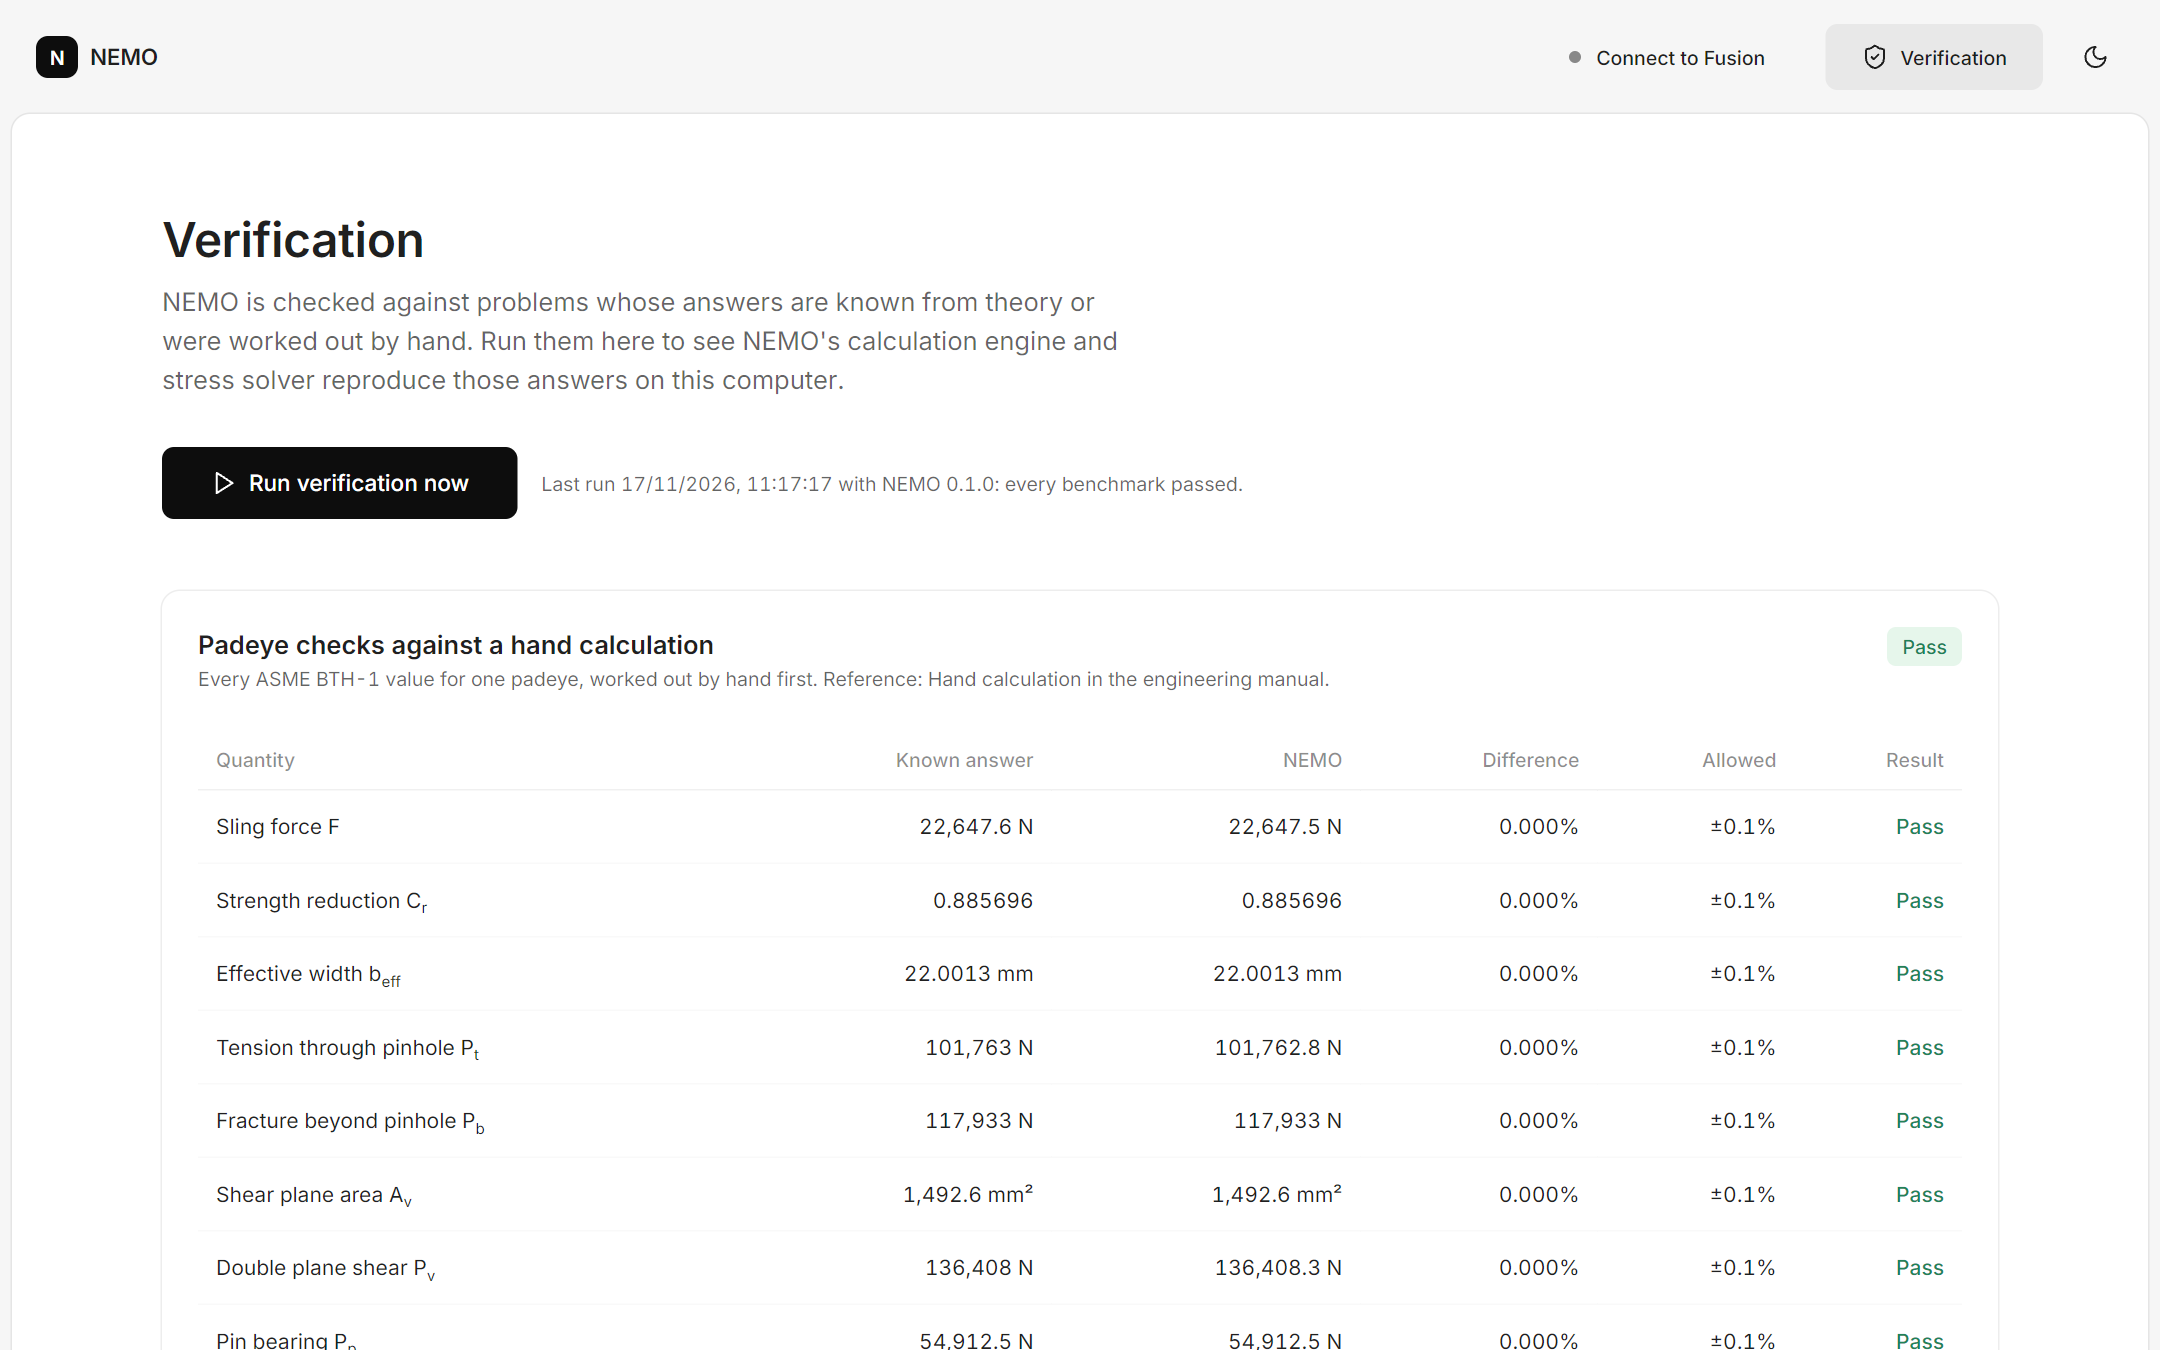
\includegraphics[width=0.8\textwidth]{images/app-verification.png}
\caption{Verification page of the application after a run}
\label{fig:app-verification}
\end{figure}

\section{Case study 1: engine room lift padeye}
\label{sec:padeye-results}

\subsection{Loads}

A 5~t load lifted on two padeyes with slings at 60$^\circ$ gives, from
Equation~\eqref{eq:padeye-loads}, $W = 49.03$~kN, $V = 24.52$~kN per padeye
and a sling force $F = 28.31$~kN, or 2.887~t. The in-plane horizontal part is
$H = 14.15$~kN and the sideways allowance $Q = 1.415$~kN. The smallest shackle
rated for 2.887~t is the 3.25~t Crosby G-2130, with a 19.1~mm pin and a
26.9~mm jaw.

\subsection{Designs}

The search tried 36 combinations of shackle, plate and cheek thickness across
the three targets and evaluated 19,389 designs. Table~\ref{tab:padeye-designs}
gives the three designs it kept and Figure~\ref{fig:padeye-model} shows the
lightest.

\begin{table}[H]
\centering
\caption{Padeye designs for the 5~t engine room lift}
\label{tab:padeye-designs}
\small
\begin{tabularx}{\textwidth}{Xrrr}
\toprule
& \textbf{Lightest} & \textbf{Balanced} & \textbf{Extra margin}\\
\midrule
Target maximum use & 100\% & 85\% & 70\%\\
Shackle (Crosby G-2130) & 3.25~t & 4.75~t & 4.75~t\\
Main plate (mm) & 6 & 8 & 8\\
Cheek plates (mm) & $2 \times 6$ & $2 \times 6$ & $2 \times 6$\\
Head radius $R$ (mm) & 21 & 25 & 22\\
Cheek radius $R_c$ (mm) & 21 & 22 & 22\\
Hole diameter $D_h$ (mm) & 20.5 & 23.5 & 23.5\\
Hole height $h$ (mm) & 39 & 45 & 45\\
Base length $L$ (mm) & 140 & 140 & 160\\
Base weld leg (mm) & 4 & 5 & 5\\
Cheek weld leg (mm) & 3 & 5 & 5\\
Steel mass (kg) & 0.305 & 0.432 & 0.447\\
Governing check & Base weld, 98.0\% & Base weld, 81.0\% & Base weld, 67.3\%\\
FEA peak von Mises (MPa) & 228.1 & 189.6 & 200.4\\
Factor of safety on yield & 1.56 & 1.87 & 1.77\\
\bottomrule
\end{tabularx}
\end{table}

The balanced design is 42\% heavier than the lightest, though its target is
only 15 points lower. The jump comes from the shackle. The shackle rating is a
strength check, and the 3.25~t shackle runs at 88.8\% of its working load
limit. That is above the 85\% target, so the balanced design has to move to
the 4.75~t shackle. The larger pin, 22.4~mm, needs a 23.5~mm hole, a wider
jaw fill and a taller head, and the plate goes from 6~mm to 8~mm to fill the
31.8~mm jaw. The extra margin design then costs only 15~g more. This shows how
discrete catalogue steps, not the continuous dimensions, set the mass of small
lifting details.

Table~\ref{tab:padeye-checks} lists every check on the lightest design. The
base weld governs at 98.0\%, followed by the shackle rating at 88.8\% and the
combined stress at the base at 88.1\%. The head checks are between 56\% and
72\%. The cheek plates were chosen because they let a 6~mm main plate fill the
jaw and carry the pin bearing. Without them, the main plate would have to be
thick enough on its own, and a thicker plate is heavier along its whole base.

\begin{table}[H]
\centering
\caption{Checks on the lightest padeye}
\label{tab:padeye-checks}
\small
\begin{tabularx}{\textwidth}{>{\raggedright\arraybackslash}Xrrlr>{\raggedright\arraybackslash}p{0.24\textwidth}}
\toprule
\textbf{Check} & \textbf{Demand} & \textbf{Capacity} & \textbf{Unit} & \textbf{Use} & \textbf{Basis}\\
\midrule
Tearing across the sides of the hole & 28,309 & 45,478 & N & 62.2\% & BTH-1\\
Splitting above the hole & 28,309 & 39,419 & N & 71.8\% & BTH-1\\
Shearing out above the hole & 28,309 & 42,628 & N & 66.4\% & BTH-1\\
Crushing under the shackle pin & 28,309 & 50,854 & N & 55.7\% & BTH-1\\
Pulling and bending at the base & 0.881 & 1 & ratio & 88.1\% & BTH-1\\
Shear at the base & 16.9 & 68.3 & MPa & 24.8\% & BTH-1\\
Base weld strength & 78.7 & 80.3 & MPa & 98.0\% & BTH-1\\
Cheek plate welds & 33.7 & 80.3 & MPa & 42.0\% & BTH-1\\
Shackle is rated for the load & 2.887 & 3.25 & t & 88.8\% & Crosby WLL\\
Hole is big enough for the pin & 20.1 & 20.5 & mm & 98.0\% & Practice\\
Padeye fits inside the shackle & 20 & 26.9 & mm & 74.3\% & Practice\\
Pin fits the hole closely (advice) & 0.90 & 0.932 & ratio & 96.6\% & BTH-1 commentary\\
Padeye fills the shackle jaw (advice) & 16.1 & 18 & mm & 89.7\% & Practice\\
Base weld size (advice) & 3 & 4 & mm & 75.0\% & AWS D1.1\\
Cheek weld size (advice) & 3 & 3 & mm & 100.0\% & AWS D1.1\\
\bottomrule
\end{tabularx}
\end{table}

Figure~\ref{fig:padeye-search} shows every design the search tried for the
lightest target, by mass and highest use. Most of the designs tried pass. None
has a highest use below 88.8\%, the use of the 3.25~t shackle, which no change
to the plate can lower. The designs that fail are the lightest ones, above the
100\% line, and the chosen design sits at the left end of the passing set.

\begin{figure}[H]
\centering
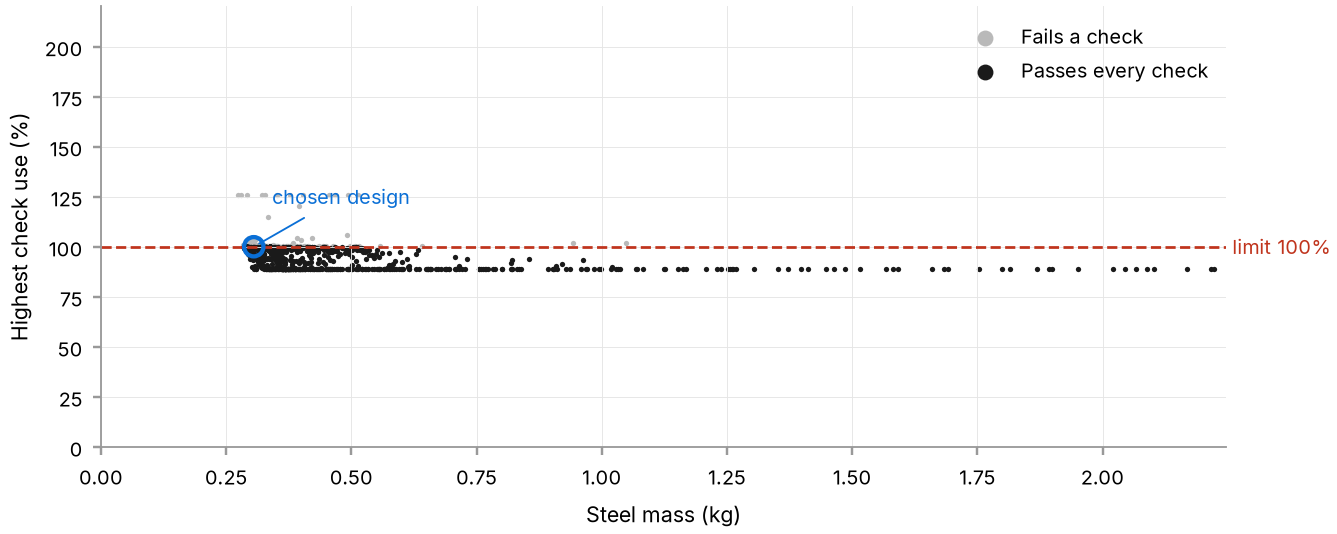
\includegraphics[width=0.75\textwidth]{images/padeye-search.png}
\caption{Designs tried by the search for the lightest padeye}
\label{fig:padeye-search}
\end{figure}

\subsection{Finite element results}

Figure~\ref{fig:padeye-stress} shows the von Mises stress in the lightest
padeye. The highest stress is at the sides of the hole, where the pin load
spreads round the head, as the BTH-1 tension and fracture checks assume.
Table~\ref{tab:padeye-fea} gives the three meshes. The peak in the head
region changed by 0.20\% between the two finest meshes, well inside the 5\%
criterion. The applied load matched the design forces, 14,155~N, 1,415~N and
24,516~N in the three directions, and the force balance error was below
$10^{-12}$ on every mesh.

\begin{figure}[H]
\centering
\begin{subfigure}{0.49\textwidth}
\centering
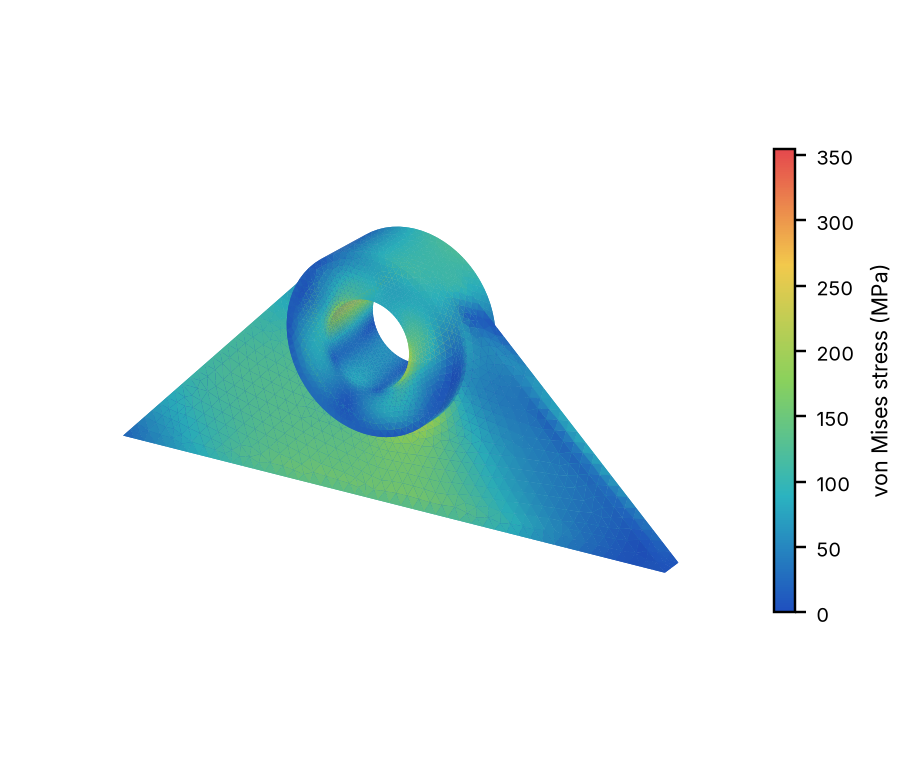
\includegraphics[width=\textwidth]{images/padeye-stress.png}
\caption{Whole padeye}
\end{subfigure}
\hfill
\begin{subfigure}{0.49\textwidth}
\centering
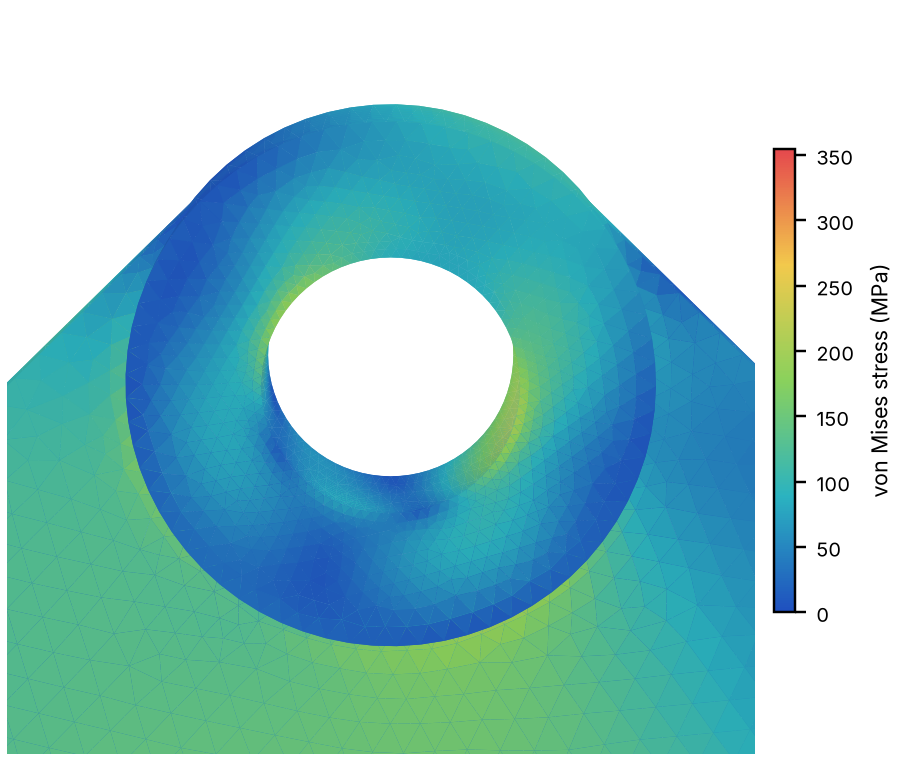
\includegraphics[width=\textwidth]{images/padeye-stress-head.png}
\caption{Head and hole}
\end{subfigure}
\caption{Von Mises stress in the lightest padeye under the 28.3~kN sling force}
\label{fig:padeye-stress}
\end{figure}

\begin{table}[H]
\centering
\caption{Mesh study of the lightest padeye}
\label{tab:padeye-fea}
\small
\begin{tabular}{lrrr}
\toprule
& \textbf{Mesh 1} & \textbf{Mesh 2} & \textbf{Mesh 3}\\
\midrule
Element size, general / at hole (mm) & 6.00 / 1.61 & 4.20 / 1.13 & 3.00 / 0.81\\
Elements & 6,487 & 17,200 & 44,271\\
Unknowns & 34,986 & 86,325 & 209,763\\
Peak von Mises in head region (MPa) & 227.56 & 227.63 & 228.09\\
Largest displacement (mm) & 0.1647 & 0.1662 & 0.1671\\
Force balance error & $1.0\times10^{-12}$ & $4.1\times10^{-13}$ & $2.1\times10^{-13}$\\
Solve time (s) & 4.2 & 12.9 & 26.9\\
\bottomrule
\end{tabular}
\end{table}

The peak of 228~MPa is 64\% of the 355~MPa yield stress, a factor of safety
of 1.56, while the code checks report the design at 98\% use. The two numbers
measure different things and do not conflict. BTH-1 category~B applies a
design factor of 3.0 to strength, and 3.6 to pin-connected plates, so a
design at 100\% use is still far from failure. The finite element peak is an
elastic local stress at the edge of the hole, which includes the stress
concentration that the code capacities allow for through their empirical
coefficients. Its role is to confirm the load path and to show that no part of
the plate yields at the working load. The governing weld is not in the solid
model, because the model treats the plate and deck as joined. The weld check
therefore rests on the hand calculation alone.

\subsection{Response to load and sling angle}

Figure~\ref{fig:padeye-load-sweep} shows the mass of the lightest padeye for
loads of 1~t to 40~t at three sling angles. The mass rises faster than the
load. At 40~t the padeye for 45$^\circ$ slings weighs 7.50~kg, against 5.26~kg
at 60$^\circ$ and 3.34~kg at 90$^\circ$, because a flatter sling raises both
the sling force and the bending at the base.

\begin{figure}[H]
\centering
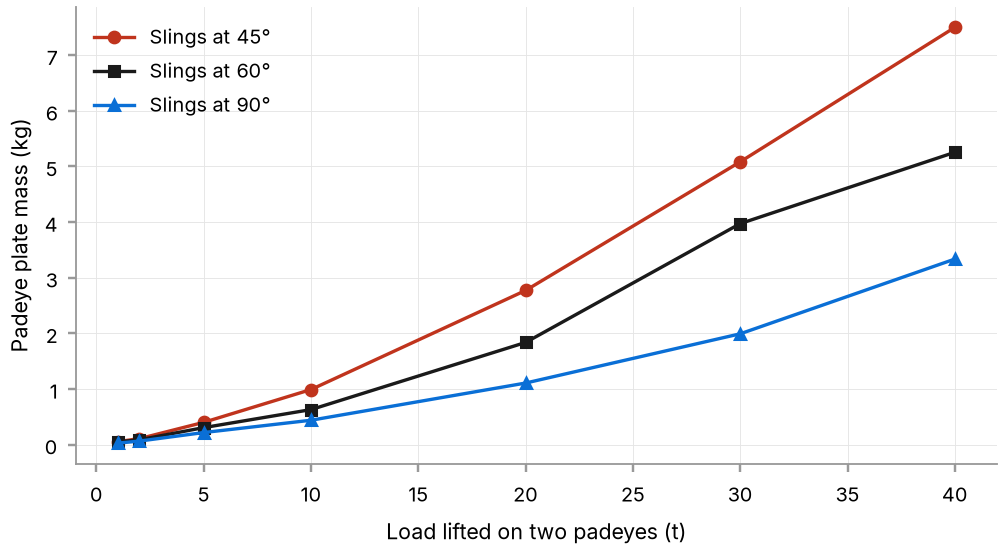
\includegraphics[width=0.75\textwidth]{images/padeye-load-sweep.png}
\caption{Mass of the lightest padeye against the load lifted on two padeyes}
\label{fig:padeye-load-sweep}
\end{figure}

The governing check changes along the sweep. At 1~t and 2~t the base weld
governs, except with vertical slings, where the shackle rating governs at
100\% because the sling force equals the working load limit of a standard
size. At most loads between 5~t and 20~t the base weld or the combined stress
at the base governs. Splitting above the hole governs from 20~t at
45$^\circ$ and from 30~t at 60$^\circ$ and 90$^\circ$, at 96\% to 100\%. It
also governs the 5~t padeye on vertical slings, which uses a 20~mm plate
without cheeks. The curves are not smooth because the plate thickness and the
shackle size change in steps. At 60$^\circ$, for example, the 2~t padeye uses
a 12~mm plate without cheeks and the 5~t padeye a 6~mm plate with cheeks.

\section{Case study 2: engine room seawater line bracket}
\label{sec:bracket-results}

\subsection{Loads}

An NPS~4 standard-wall carbon steel pipe, 114.3~mm by 6.02~mm, weighs
16.08~kg/m, and its sea water adds 8.42~kg/m. The weight per metre is
240.2~N/m. With 3~m spacing and the continuity factor of 1.25, one bracket
carries 0.901~kN. The ship motion raises this to 1.80~kN downward, with
0.72~kN across the pipe and 0.54~kN of friction along it.

\subsection{Design}

The search found one design. The lightest bracket uses so little of its
strength that it already meets the 85\% and 70\% targets, so the other two
searches returned the same design and the tool offered it alone.
Table~\ref{tab:bracket-design} gives the design and
Table~\ref{tab:bracket-checks-result} its checks. The search ran 63
combinations of seat and knee thickness over the three targets. Lower-bound
pruning skipped 60 of them, and only 300 designs had to be evaluated.

\begin{table}[H]
\centering
\caption{Pipe support bracket for the NPS~4 seawater line}
\label{tab:bracket-design}
\small
\begin{tabular}{lr}
\toprule
Seat plate, length by width by thickness (mm) & $195 \times 50 \times 6$\\
Knees, two, thickness (mm) & 6\\
Knee depth at the bulkhead (mm) & 60\\
Pipe centre from the bulkhead (mm) & 107.15\\
U-bolt & M12, class 4.6, galvanised\\
Fillet welds, bulkhead and knee to seat (mm) & 3 and 3\\
Steel mass (kg) & 0.996\\
Governing strength check & Welds to the bulkhead, 25.4\%\\
FEA peak von Mises, away from the bulkhead (MPa) & 34.65\\
Hand stress, seat between the knees (MPa) & 37.53\\
\bottomrule
\end{tabular}
\end{table}

\begin{table}[H]
\centering
\caption{Checks on the bracket and the pipe span}
\label{tab:bracket-checks-result}
\small
\begin{tabularx}{\textwidth}{>{\raggedright\arraybackslash}Xrrlr}
\toprule
\textbf{Check} & \textbf{Demand} & \textbf{Capacity} & \textbf{Unit} & \textbf{Use}\\
\midrule
Bending along the bracket arm & 0.191 & 1 & ratio & 19.1\%\\
Shear in the arm & 2.89 & 84.4 & MPa & 3.4\%\\
Welds to the bulkhead & 36.7 & 144.6 & MPa & 25.4\%\\
Knee-to-seat welds & 3.32 & 144.6 & MPa & 2.3\%\\
Seat plate between the knees & 37.5 & 211.1 & MPa & 17.8\%\\
U-bolt legs & 0.003 & 1 & ratio & 0.3\%\\
Bracket deflection under the pipe & 0.016 & 1 & mm & 1.6\%\\
Knee free edge (advice) & 204 & 300 & mm & 68.0\%\\
Bulkhead and knee weld sizes (advice) & 3 & 3 & mm & 100.0\%\\
\midrule
Pipe span clear of vibration & 0.20 & 0.265 & ratio & 75.5\%\\
Pipe bending between supports & 8.84 & 143.7 & MPa & 6.2\%\\
Pipe sag between supports (advice) & 0.415 & 2.5 & mm & 16.6\%\\
Spacing within the recommended maximum (advice) & 3.0 & 2.3 & m & 130.4\%\\
\bottomrule
\end{tabularx}
\end{table}

No strength check exceeds 26\%. The bracket is sized by minimums instead.
The plates are the thinnest in the stock list, the welds are the AWS minimum of
3~mm, the U-bolt is the smallest \NEMO{} allows for this pipe size, and the seat
must be wide enough for the U-bolt holes. A search that only minimised mass
under strength checks would have produced plates thinner than the yard holds.
This is why the stock list and the fit rules form part of the design method
and are not applied afterwards.

\subsection{Pipe span}

The span check gives a different picture. The first natural frequency of the
3~m span is 27.57~Hz. The excitations are 2.0~Hz from shaft rotation, 8.0~Hz
from blade rate, 16.0~Hz from twice blade rate, 12.5~Hz from engine rotation
and 37.5~Hz from engine firing. The nearest is the firing frequency, 26.5\%
away, so the span passes the 20\% margin. But the recommended maximum spacing
is 2.3~m. Below that spacing the span frequency stays at least 20\% above every
excitation. The stress limit alone would allow 12.1~m and the sag limit
4.7~m. Vibration, not strength or sag, sets the spacing of these supports.

Figure~\ref{fig:bracket-span} shows the natural frequency against spacing,
with a band of $\pm 20\%$ round each excitation. Table~\ref{tab:span-sweep}
gives the points. The result is not monotonic. A spacing of 2.5~m fails,
because its 39.7~Hz is only 5.9\% from firing. The 3~m and 3.5~m spans pass,
because they fall in the gap between twice blade rate and firing. The 4~m span
fails again, 3.1\% from twice blade rate. A designer who shortened a 3~m span
to 2.5~m to be safe would move it into resonance. The recommended spacing of
2.3~m avoids this by keeping the span above all the excitations.

\begin{figure}[H]
\centering
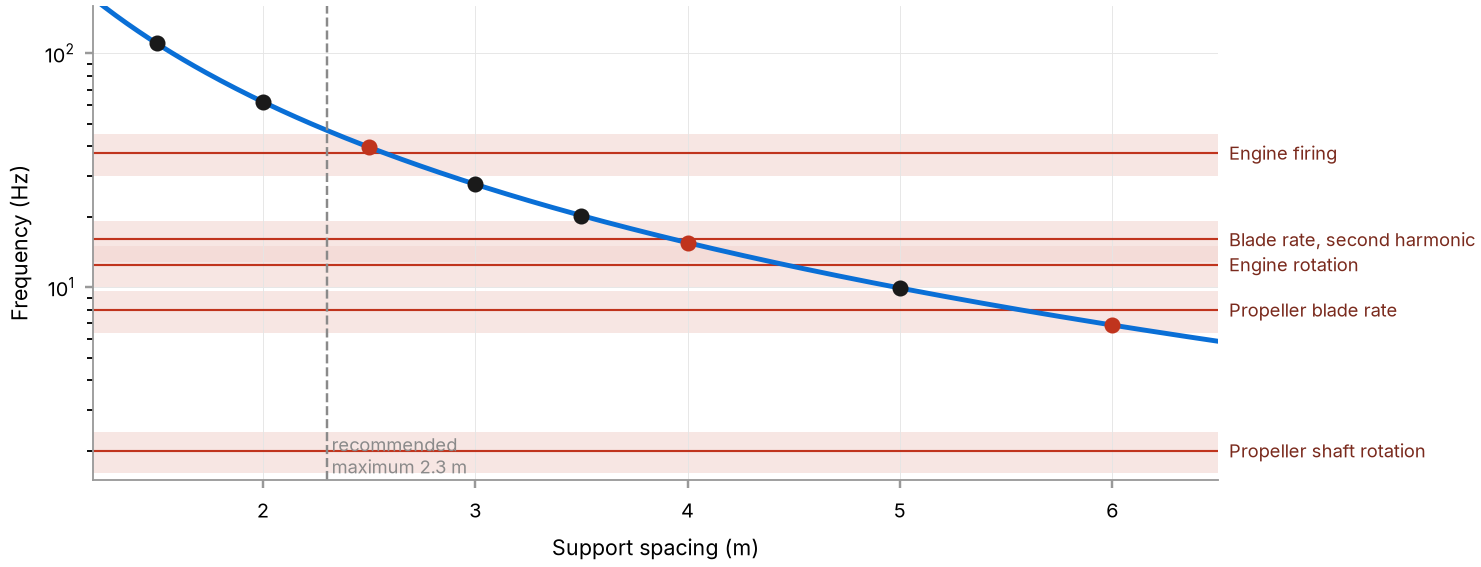
\includegraphics[width=\textwidth]{images/bracket-span-frequency.png}
\caption{Natural frequency of the NPS~4 span against support spacing, with
$\pm 20\%$ bands round each excitation. Red points fail the margin}
\label{fig:bracket-span}
\end{figure}

\begin{table}[H]
\centering
\caption{Pipe span against support spacing, NPS~4 seawater line}
\label{tab:span-sweep}
\small
\begin{tabular}{rrlrrl}
\toprule
\textbf{Spacing (m)} & \textbf{$f_n$ (Hz)} & \textbf{Nearest excitation} & \textbf{Margin} & \textbf{Stress (MPa)} & \textbf{Result}\\
\midrule
1.5 & 110.28 & Engine firing & 194.1\% & 2.2 & Passes\\
2.0 & 62.03 & Engine firing & 65.4\% & 3.9 & Passes\\
2.5 & 39.70 & Engine firing & 5.9\% & 6.1 & Fails\\
3.0 & 27.57 & Engine firing & 26.5\% & 8.8 & Passes\\
3.5 & 20.25 & Twice blade rate & 26.6\% & 12.0 & Passes\\
4.0 & 15.51 & Twice blade rate & 3.1\% & 15.7 & Fails\\
5.0 & 9.92 & Engine rotation & 20.6\% & 24.6 & Passes\\
6.0 & 6.89 & Blade rate & 13.8\% & 35.4 & Fails\\
\bottomrule
\end{tabular}
\end{table}

Figure~\ref{fig:bracket-size-sweep} repeats the case for pipe sizes NPS~2 to
NPS~12 at 3~m spacing. The recommended spacing rises from 1.7~m to 3.7~m,
because the stiffness of a pipe grows faster with diameter than its mass does.
It is set by frequency at every size. The bracket mass rises from 0.61~kg to
4.24~kg. The governing strength check moves from the bulkhead welds, at 9\% for
NPS~2, to the seat plate between the knees from NPS~10, at 82\%.

\begin{figure}[H]
\centering
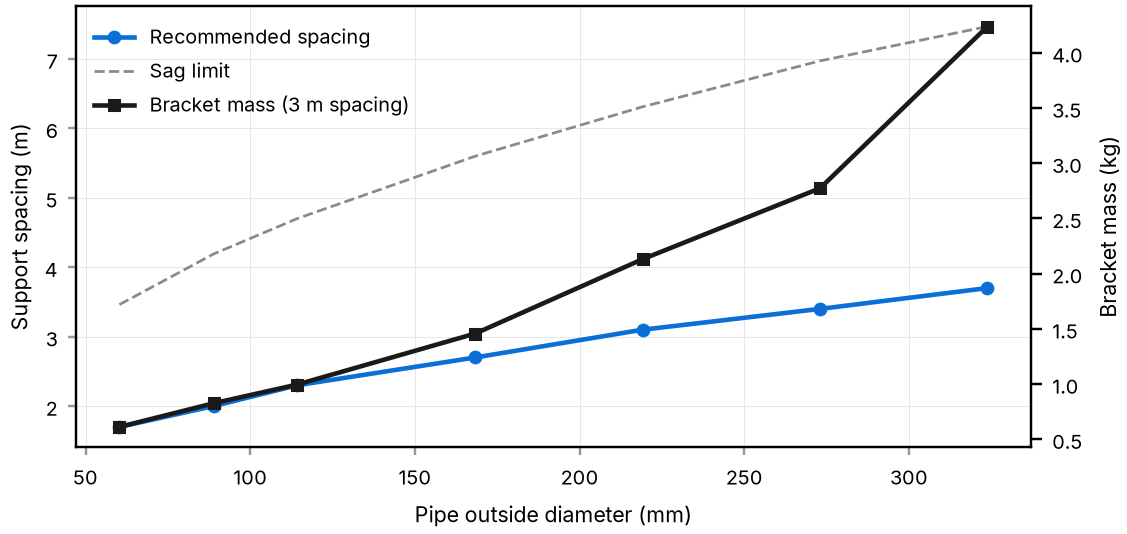
\includegraphics[width=0.8\textwidth]{images/bracket-size-sweep.png}
\caption{Recommended spacing and bracket mass against pipe size}
\label{fig:bracket-size-sweep}
\end{figure}

\subsection{Finite element results}

The peak von Mises stress away from the bulkhead face was 34.65~MPa, 7.7\%
below the hand value of 37.53~MPa for the seat plate between the knees
(Figure~\ref{fig:bracket-stress}). The hand model is a simply supported strip,
which ignores the restraint the knees give the seat edges, so it should be
higher. The peak changed by 0.54\% between the two finest meshes. The highest
stress anywhere in the model rose from 36.2~MPa to 47.6~MPa as the mesh was
refined. That value sits at the fixed edge against the bulkhead, where the
singularity described in Section~\ref{sec:fea} makes it meaningless, and the
assessed region excludes it for this reason. With a peak of 35~MPa against a
235~MPa yield, the factor of safety is 6.8.

\begin{figure}[H]
\centering
\begin{subfigure}{0.49\textwidth}
\centering
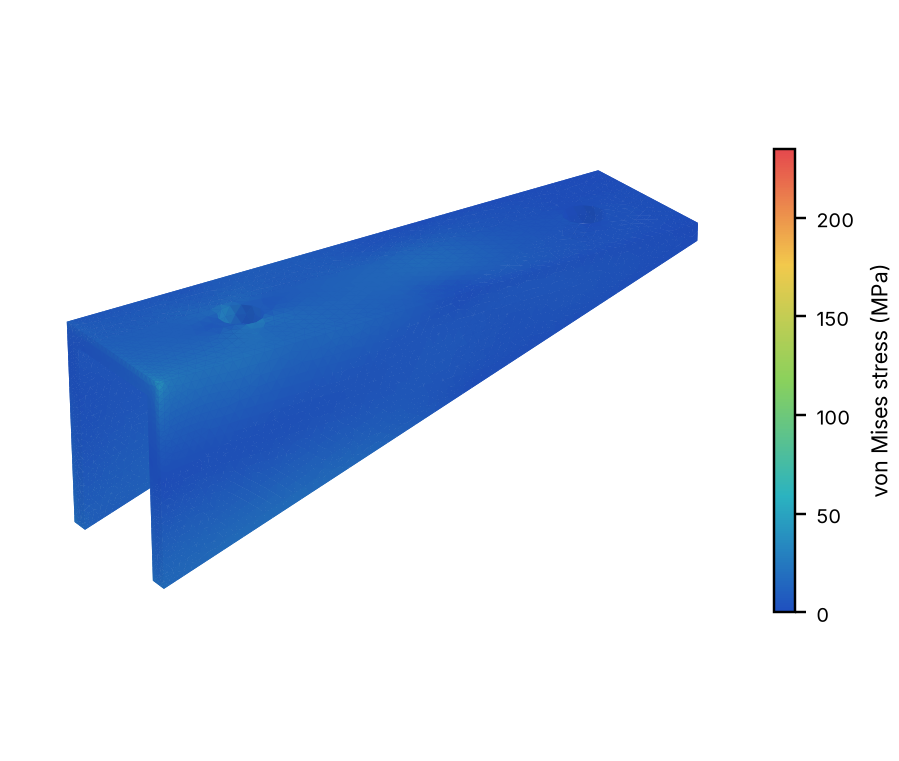
\includegraphics[width=\textwidth]{images/bracket-stress.png}
\caption{Von Mises stress}
\end{subfigure}
\hfill
\begin{subfigure}{0.49\textwidth}
\centering
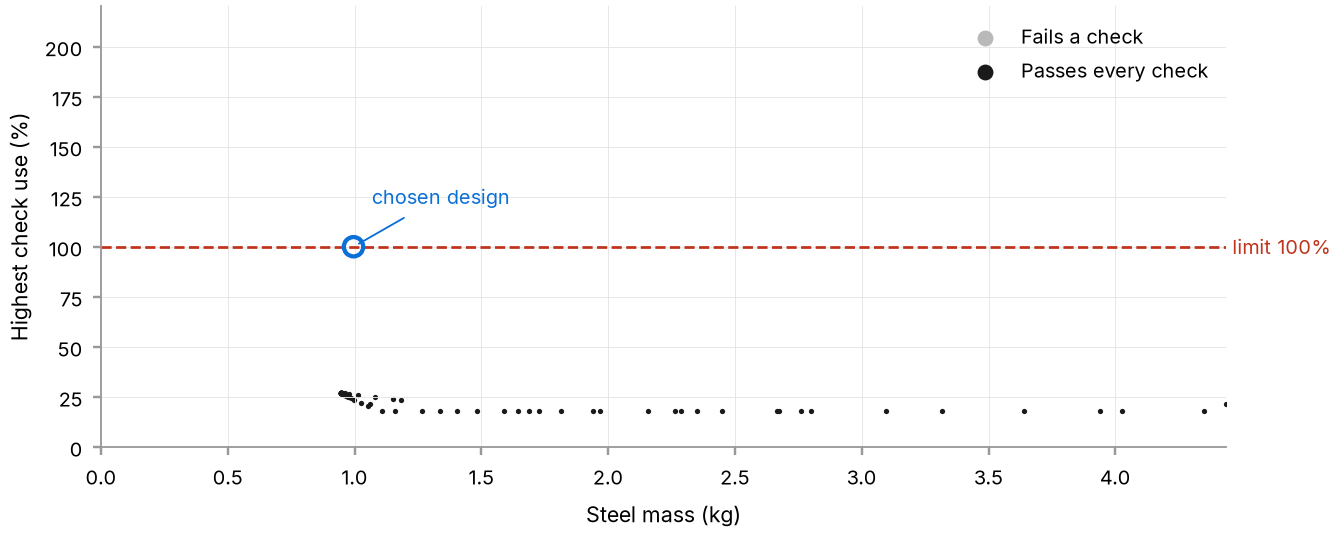
\includegraphics[width=\textwidth]{images/bracket-search.png}
\caption{Designs tried by the search}
\end{subfigure}
\caption{Bracket stress under the pipe load, and the search for the lightest
bracket}
\label{fig:bracket-stress}
\end{figure}

\section{Case study 3: patrol boat stabilizer fin}
\label{sec:fin-results}

\subsection{Loads}

At 18~knots, 9.26~m/s, the 1.4~m by 1.2~m fin has an area of 1.68~m$^2$ and
an effective aspect ratio of 2.33. Equation~\eqref{eq:whicker} gives a lift
slope of 2.708 per radian and, at 22$^\circ$, a lift coefficient of 1.090, of
which the non-linear term contributes 0.051. The foil model gives a lift of
80.49~kN. The UR S10 formula gives 66.74~kN, with $K_1 = 1.056$, $K_2 = 1.10$
and $K_3 = 0.8$. The foil model is 21\% higher and is used as the design force.
Because both methods scale with $V^2$, the ratio stays the same at every speed
(Figure~\ref{fig:fin-speed}).

The stock at 35\% chord lies 0.02$c$ aft of the 33\% centre of pressure, so the
rule minimum of $0.1Fc$ sets the twisting moment, $Q = 9.66$~kN\,m. The
bending moment is 56.34~kN\,m at the fin root and 72.44~kN\,m at the outer
bearing.

The UR S10 force formula is empirical and was written for rudders. A
stabilizer fin is a low-aspect-ratio foil, and at large angles it keeps
gaining lift through the cross-flow term of Equation~\eqref{eq:whicker}, past
the angle at which a two-dimensional section would stall
\cite{whicker1958,molland2007}. The result shows why the project derived the
load twice. Using the rule formula alone would have under-estimated the
design force by 17\% of the foil value.

\subsection{Pressure and cavitation}

The fin lift coefficient of 1.09 corresponds to a section angle of
8.5$^\circ$ on the two-dimensional NACA~0020 section. At that angle the panel
method gives the pressure distribution in Figure~\ref{fig:fin-pressure}. The
suction peak is close to the leading edge, at $C_{p,\text{min}} = -2.91$. At a
depth of 3~m and 18~knots the cavitation number is $\sigma = 2.953$, so the
advice check sits at 98.5\%. The fin is on the edge of leading-edge
cavitation at its largest angle.

\begin{figure}[H]
\centering
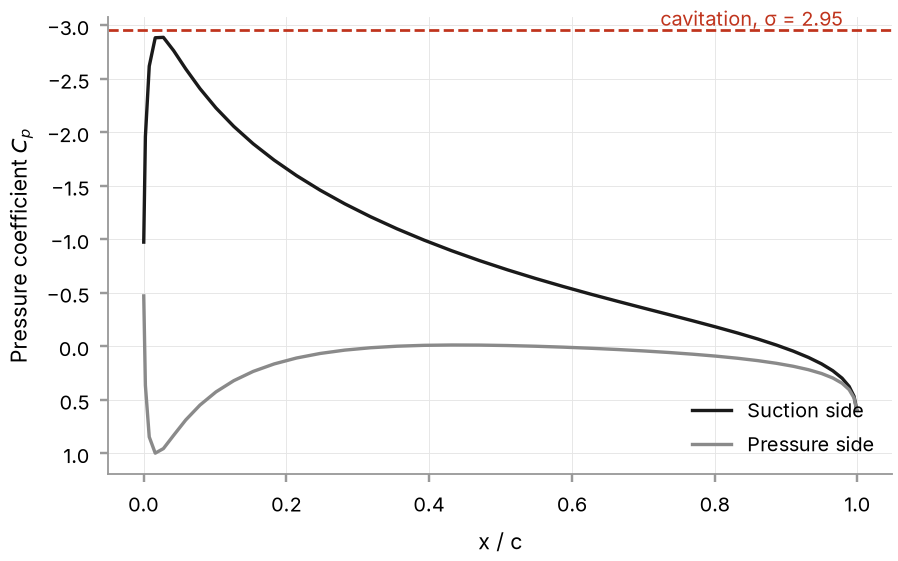
\includegraphics[width=0.65\textwidth]{images/fin-pressure.png}
\caption{Pressure on the NACA~0020 section at the angle that gives the fin's
lift coefficient, with the cavitation number at 18~knots}
\label{fig:fin-pressure}
\end{figure}

\subsection{Designs}

The search evaluated 3,780 combinations of skin, web and rib spacing over the
three targets, 1,260 per target. Table~\ref{tab:fin-designs} gives the three
designs. They differ only in the stock. The webs are at the 8~mm minimum of UR
S10, the skin is the thinnest plate in stock, 8~mm against a rule minimum of
7.54~mm, and five ribs at 350~mm pitch is the lightest arrangement in
every case, because the fin body runs at 38\% to 48\% of its strength.

\begin{table}[H]
\centering
\caption{Stabilizer fin designs at 18~knots}
\label{tab:fin-designs}
\small
\begin{tabularx}{\textwidth}{>{\raggedright\arraybackslash}Xrrr}
\toprule
& \textbf{Lightest} & \textbf{Balanced} & \textbf{Extra margin}\\
\midrule
Skin and webs (mm) & 8 & 8 & 8\\
Ribs, number at pitch (mm) & 5 at 350 & 5 at 350 & 5 at 350\\
Stock diameter (mm) & 160 & 170 & 180\\
Stock yield, EN 10083-3 (MPa) & 550 & 500 & 500\\
Mass of skin, spars and ribs (kg) & 315.4 & 315.4 & 315.4\\
Mass of stock (kg) & 142.1 & 160.4 & 179.8\\
Total mass (kg) & 457.5 & 475.8 & 495.2\\
Stock combined stress, UR S10.4.2 & 94.5\% & 78.8\% & 66.4\%\\
FEA stock stress near bearing (MPa) & 165.26 & 136.86 & 114.23\\
Beam theory at the same section (MPa) & 165.67 & 137.29 & 114.96\\
\bottomrule
\end{tabularx}
\end{table}

Table~\ref{tab:fin-checks-result} lists the checks on the lightest fin. The
stock in combined bending and twist at the outer bearing governs at 94.5\%.
The fit checks on plate thickness are close to their limits, the skin at
94.3\% of the plating formula and the webs exactly at the 8~mm minimum. The
fin body is lightly stressed, and the tip deflects 0.89~mm.

\begin{table}[H]
\centering
\caption{Checks on the lightest fin}
\label{tab:fin-checks-result}
\small
\begin{tabularx}{\textwidth}{>{\raggedright\arraybackslash}Xrrlr}
\toprule
\textbf{Check} & \textbf{Demand} & \textbf{Capacity} & \textbf{Unit} & \textbf{Use}\\
\midrule
Stock twisting, S10.4.1 & 12.0 & 110.7 & MPa & 10.9\%\\
Stock bending and twisting at the outer bearing, S10.4.2 & 181.6 & 192.1 & MPa & 94.5\%\\
Stock fits inside the foil & 160 & 214.1 & mm & 74.7\%\\
Fin body bending at the root, S10.5.1 & 55.7 & 146.1 & MPa & 38.1\%\\
Spar web shear at the root, S10.5.1 & 31.2 & 66.4 & MPa & 47.0\%\\
Fin skin combined stress, S10.5.1 & 56.3 & 159.4 & MPa & 35.3\%\\
Skin plate thickness, S10.5.2 & 7.54 & 8 & mm & 94.3\%\\
Spar and rib web thickness, S10.5.2 & 8 & 8 & mm & 100.0\%\\
Skin panel buckling & 55.7 & 116.5 & MPa & 47.8\%\\
Fin tip deflection & 0.89 & 10 & mm & 8.9\%\\
Cavitation at the largest fin angle (advice) & 2.91 & 2.953 & ratio & 98.5\%\\
\bottomrule
\end{tabularx}
\end{table}

The rule capacities for the stock do not change between the designs, though
the stock yield falls from 550~MPa to 500~MPa above 160~mm diameter. UR S10
caps the yield used in the material factor at $\min(0.7\sigma_T, 450)$~MPa.
With a tensile strength of 750~MPa that cap is 450~MPa, below both yields, so
$k = 0.614$ in every case and the combined limit is $118/k = 192.1$~MPa.

\subsection{Finite element results}

The stock model of the lightest design gave 165.26~MPa in the assessed region,
0.25\% below beam theory at the same section (Figure~\ref{fig:fin-stock}). The
peak changed by 0.12\% between the two finest meshes. The highest stress in
the whole model, 190.2~MPa, is at the fixed bearing face and is excluded for
the reason given in Section~\ref{sec:fea}. Against the 550~MPa yield, the
factor of safety is 3.33. The UR S10 check is far more severe than this, at
94.5\%, because its limit of 192.1~MPa is about 35\% of yield. The rule
limit, not the elastic stress, decides the stock size.

\begin{figure}[H]
\centering
\begin{subfigure}{0.49\textwidth}
\centering
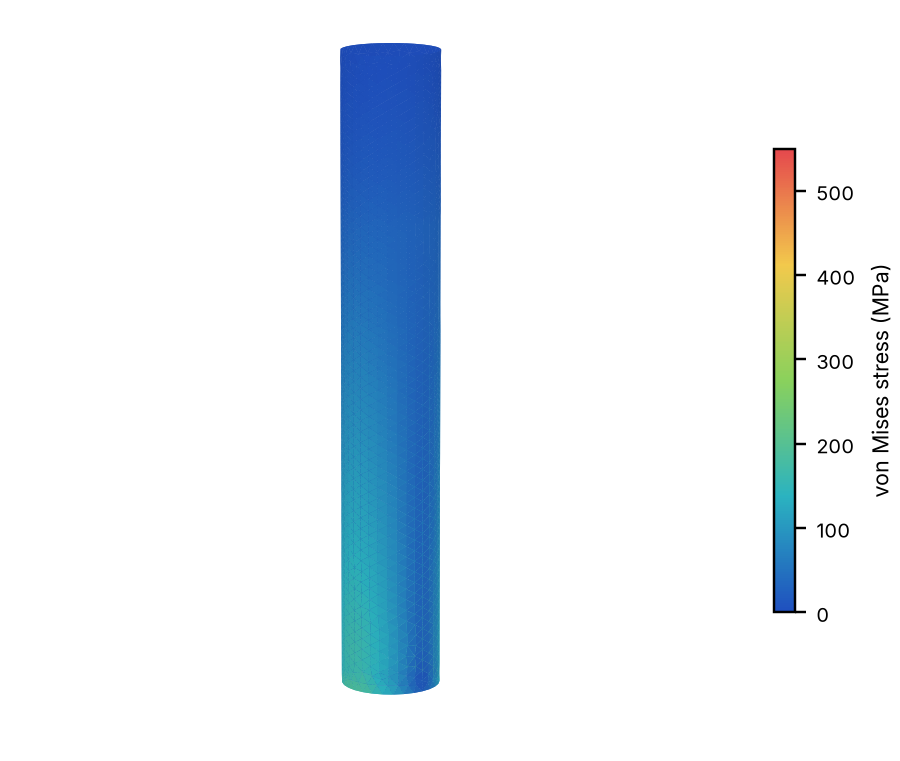
\includegraphics[width=\textwidth]{images/fin-stock-stress.png}
\caption{Von Mises stress in the stock}
\end{subfigure}
\hfill
\begin{subfigure}{0.49\textwidth}
\centering
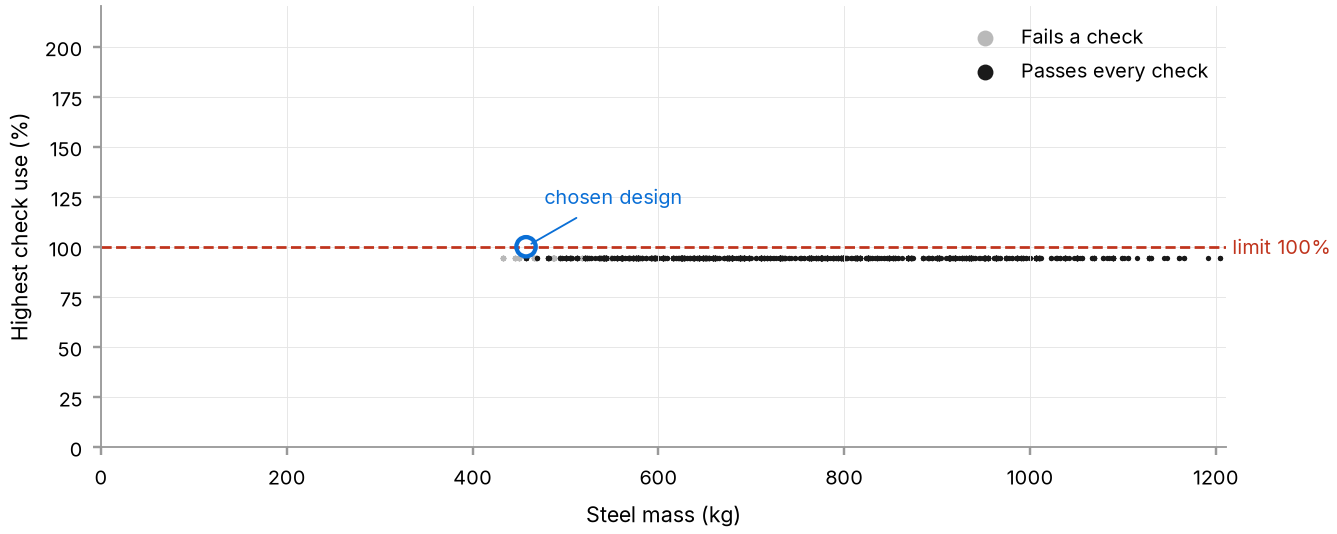
\includegraphics[width=\textwidth]{images/fin-search.png}
\caption{Designs tried by the search}
\end{subfigure}
\caption{Stock stress under the fin force and twist, and the search for the
lightest fin}
\label{fig:fin-stock}
\end{figure}

Figure~\ref{fig:convergence} brings together the mesh studies of the three
case studies. In each case the assessed peak settles on the first refinement,
and for the bracket and the fin it lies close to the hand value.

\begin{figure}[H]
\centering
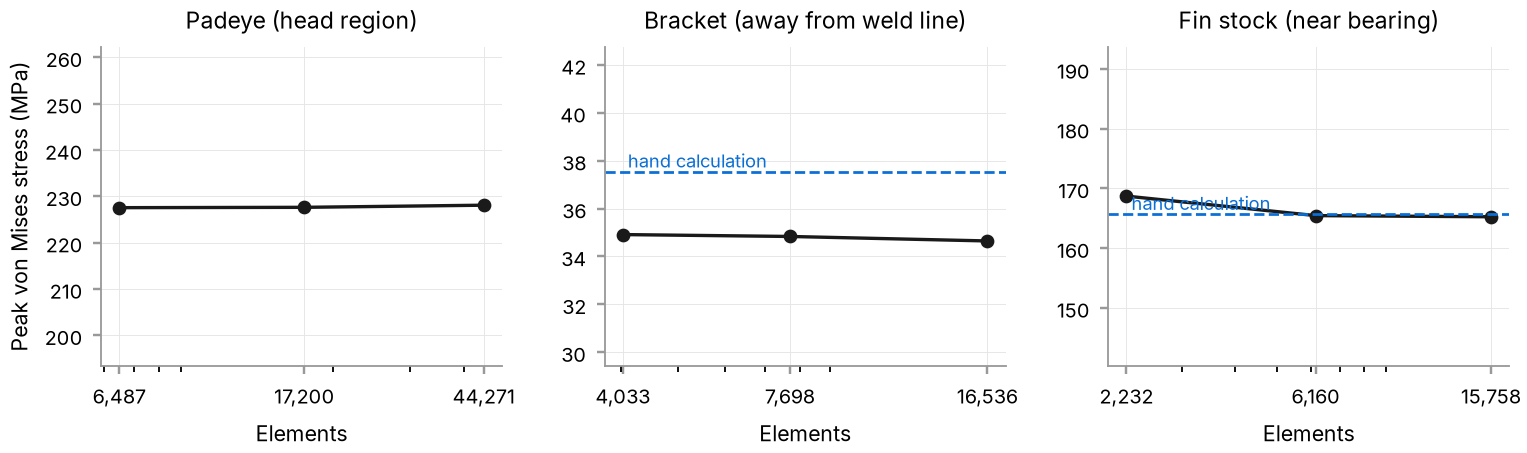
\includegraphics[width=\textwidth]{images/convergence.png}
\caption{Assessed peak stress against the number of elements for the three
lightest designs, with the hand values where they apply}
\label{fig:convergence}
\end{figure}

\subsection{Response to ship speed}

Figure~\ref{fig:fin-speed} and Figure~\ref{fig:fin-stock-sweep} show the fin
sized for speeds from 10~knots to 24~knots. The design force rises from
24.8~kN to 143.1~kN and the stock from 110~mm to 195~mm. The fin mass rises
from 370~kg to 539~kg, and nearly all of that increase is in the stock,
because the skin and webs stay at the 8~mm minimum. The cavitation number falls
with the square of speed, while $-C_{p,\text{min}}$ stays at 2.91 because the
angle is fixed. Cavitation begins between 18 and 20~knots. At 20~knots
$\sigma = 2.39$, well below 2.91. For this fin, cavitation would limit the
largest angle at high speed before the structure does.

\begin{figure}[H]
\centering
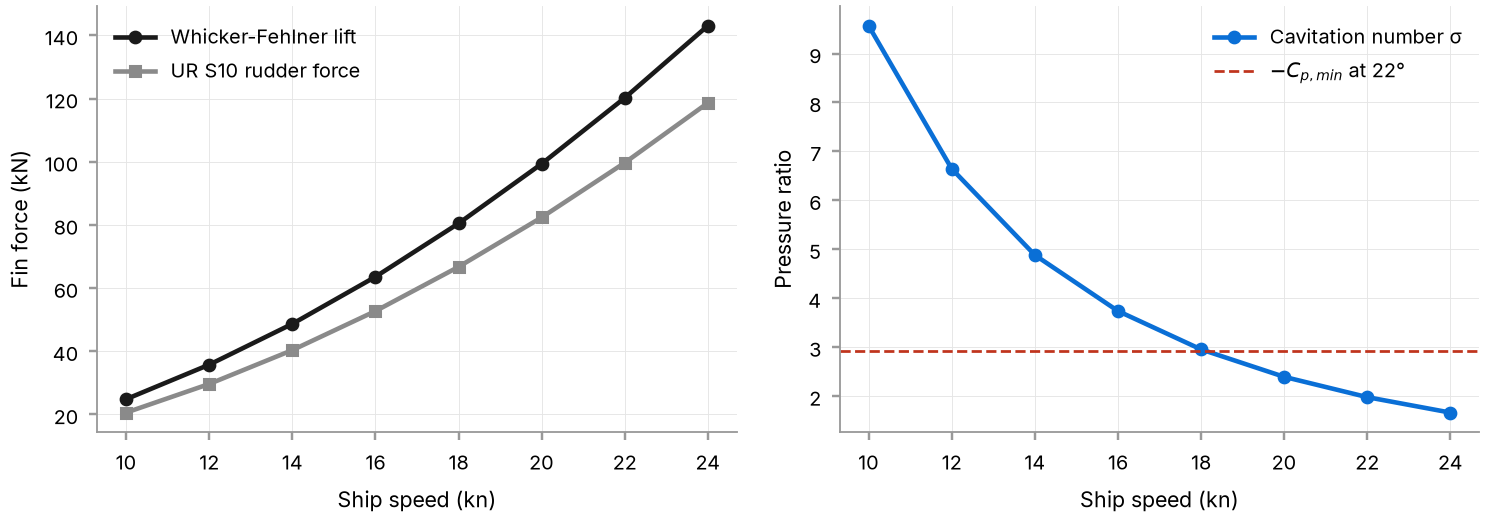
\includegraphics[width=\textwidth]{images/fin-speed-sweep.png}
\caption{Fin force from the two load methods, and cavitation number against
the lowest pressure, over ship speed}
\label{fig:fin-speed}
\end{figure}

\begin{figure}[H]
\centering
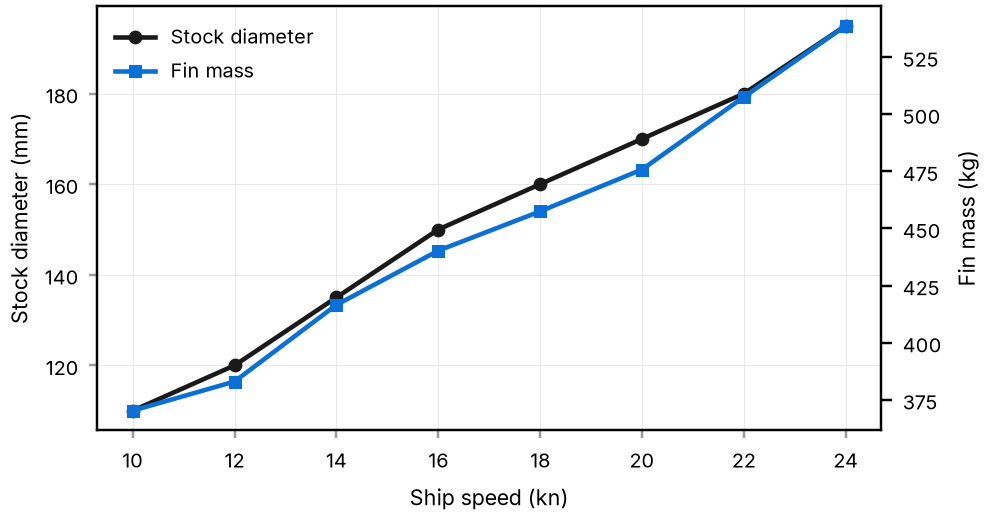
\includegraphics[width=0.7\textwidth]{images/fin-stock-sweep.png}
\caption{Stock diameter and fin mass against ship speed}
\label{fig:fin-stock-sweep}
\end{figure}

\section{Calculation package and application}
\label{sec:results-package}

Each design produced a PDF calculation package of 0.34~MB to 0.64~MB.
Figure~\ref{fig:padeye-report} shows three pages from the package of the
lightest padeye. The summary page gives the design, the loads and the
governing check. The drawing is dimensioned from the same design record as the
STEP file. The check pages show each formula with its values, its result and
its source, so that a checker can follow the calculation without the
software.

\begin{figure}[H]
\centering
\begin{subfigure}{0.32\textwidth}
\centering
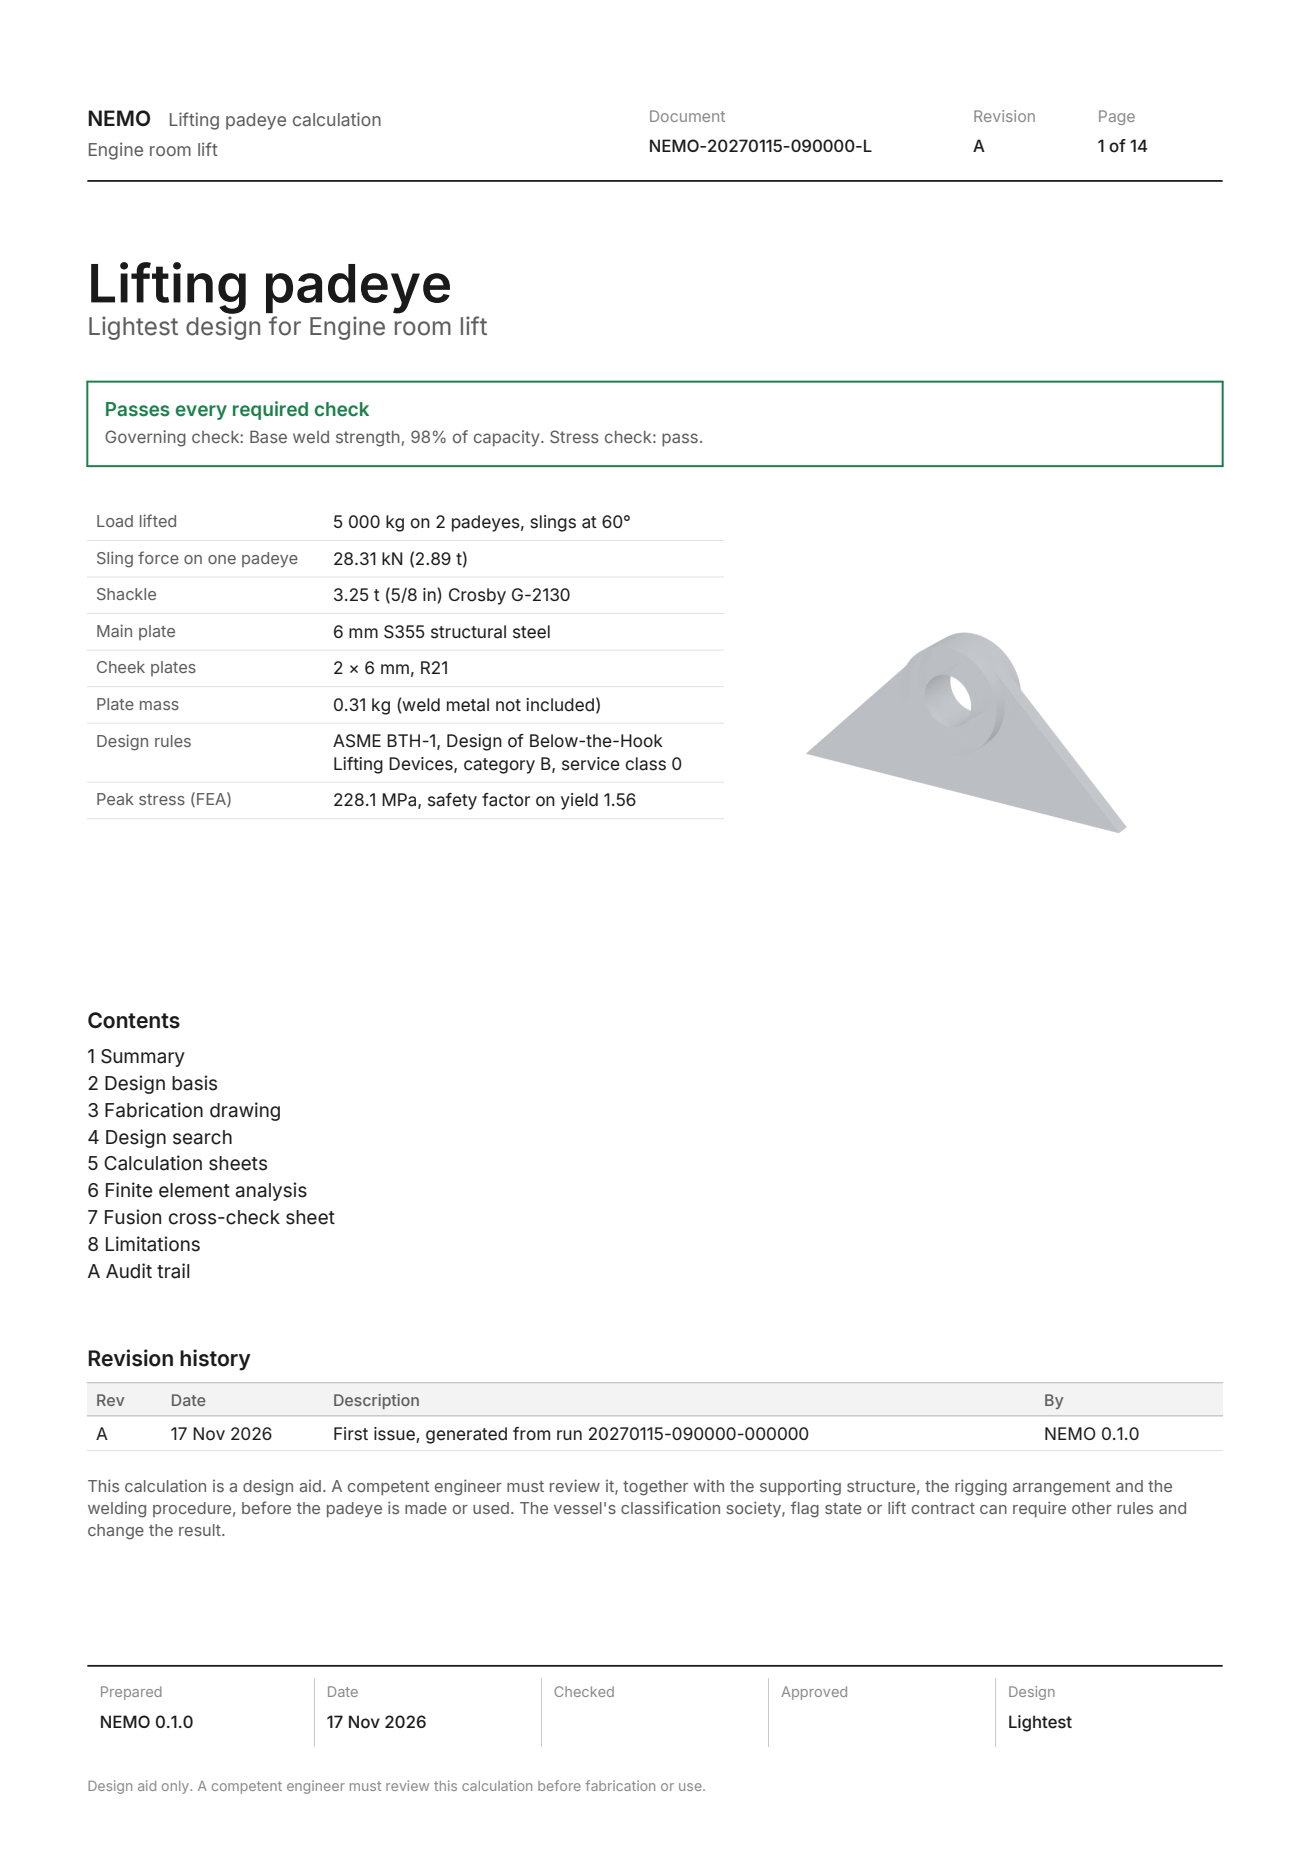
\includegraphics[width=\textwidth]{images/padeye-report-summary.png}
\caption{Summary}
\end{subfigure}
\hfill
\begin{subfigure}{0.32\textwidth}
\centering
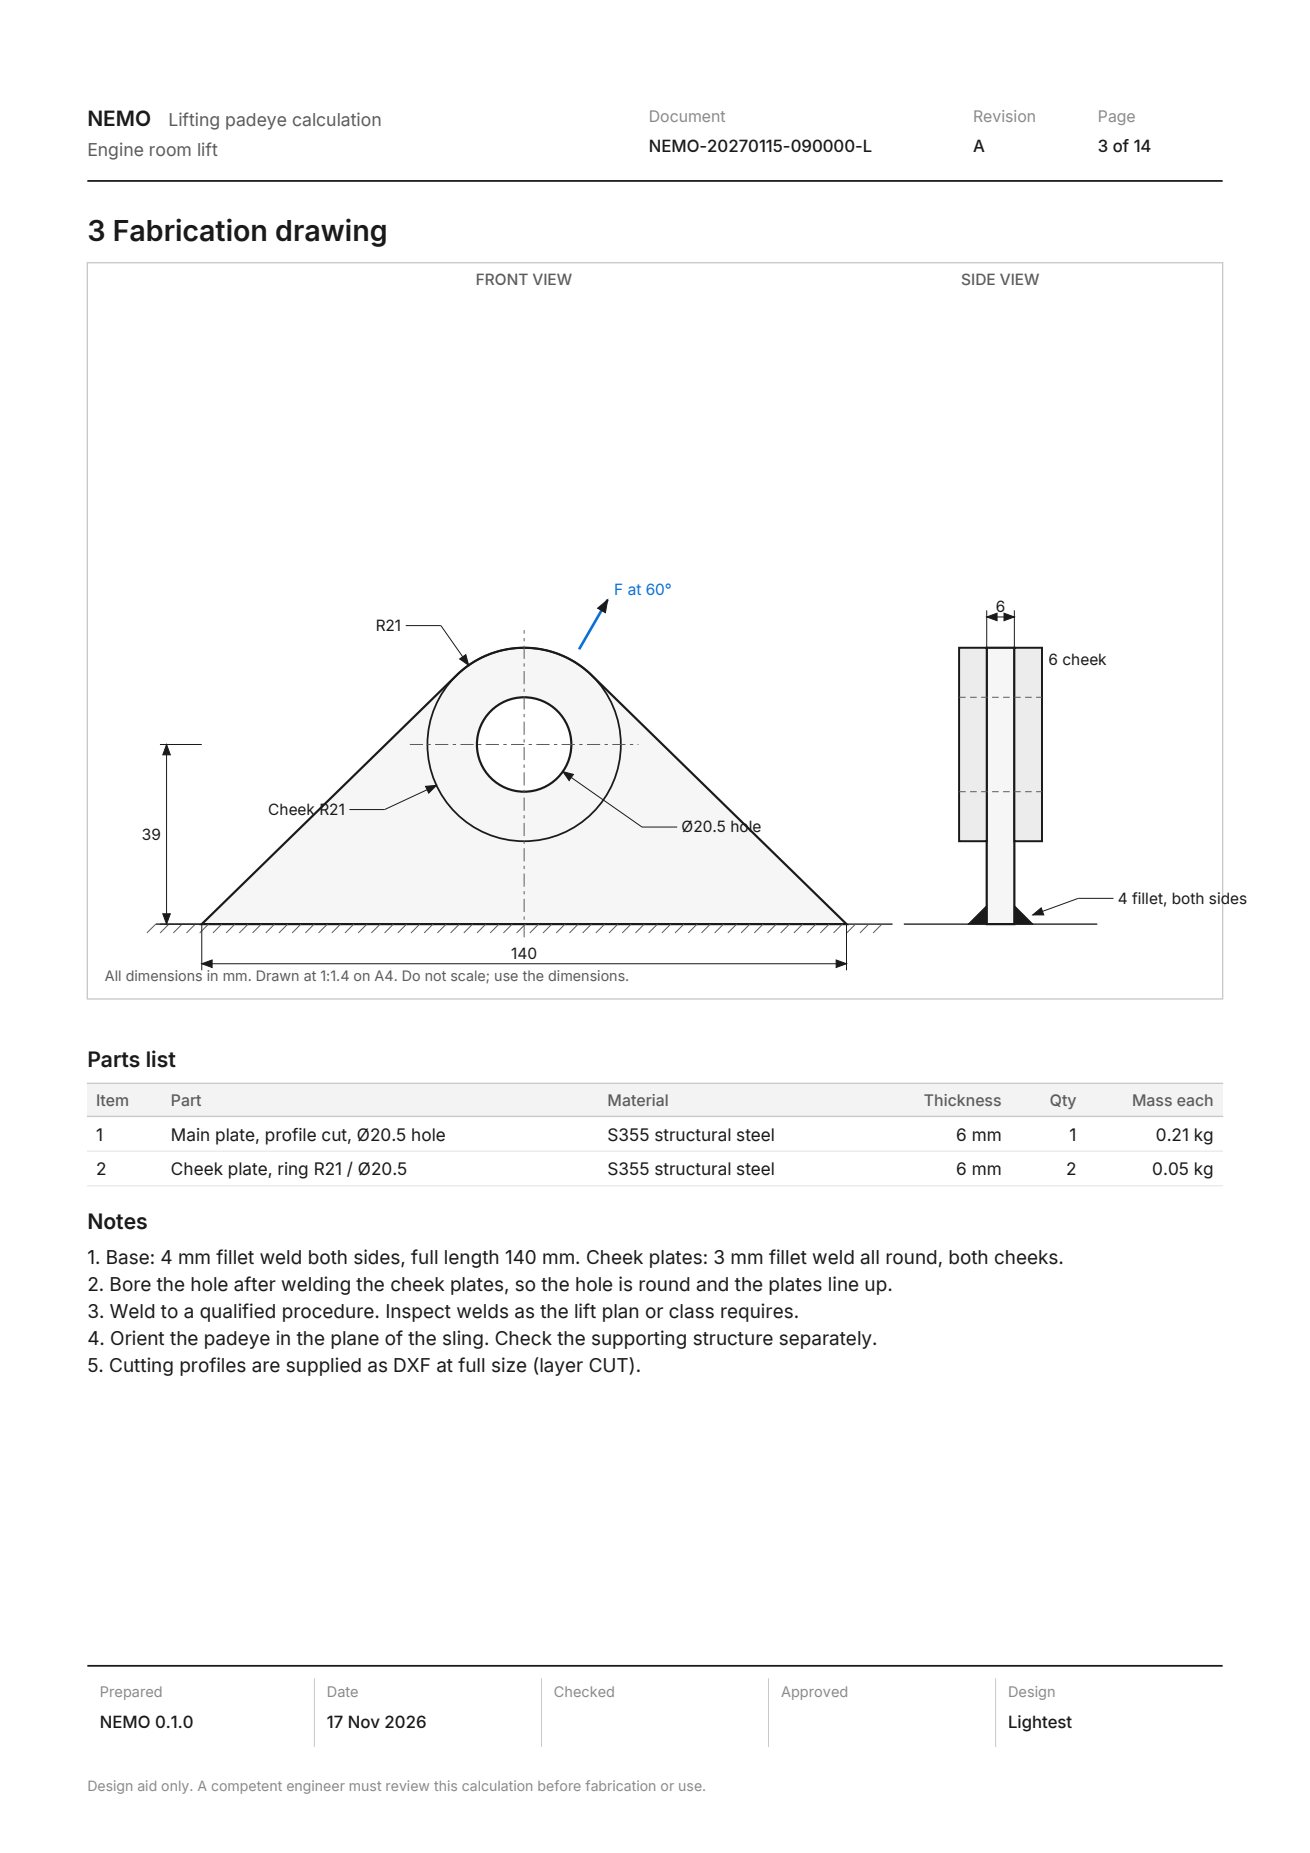
\includegraphics[width=\textwidth]{images/padeye-report-drawing.png}
\caption{Drawing}
\end{subfigure}
\hfill
\begin{subfigure}{0.32\textwidth}
\centering
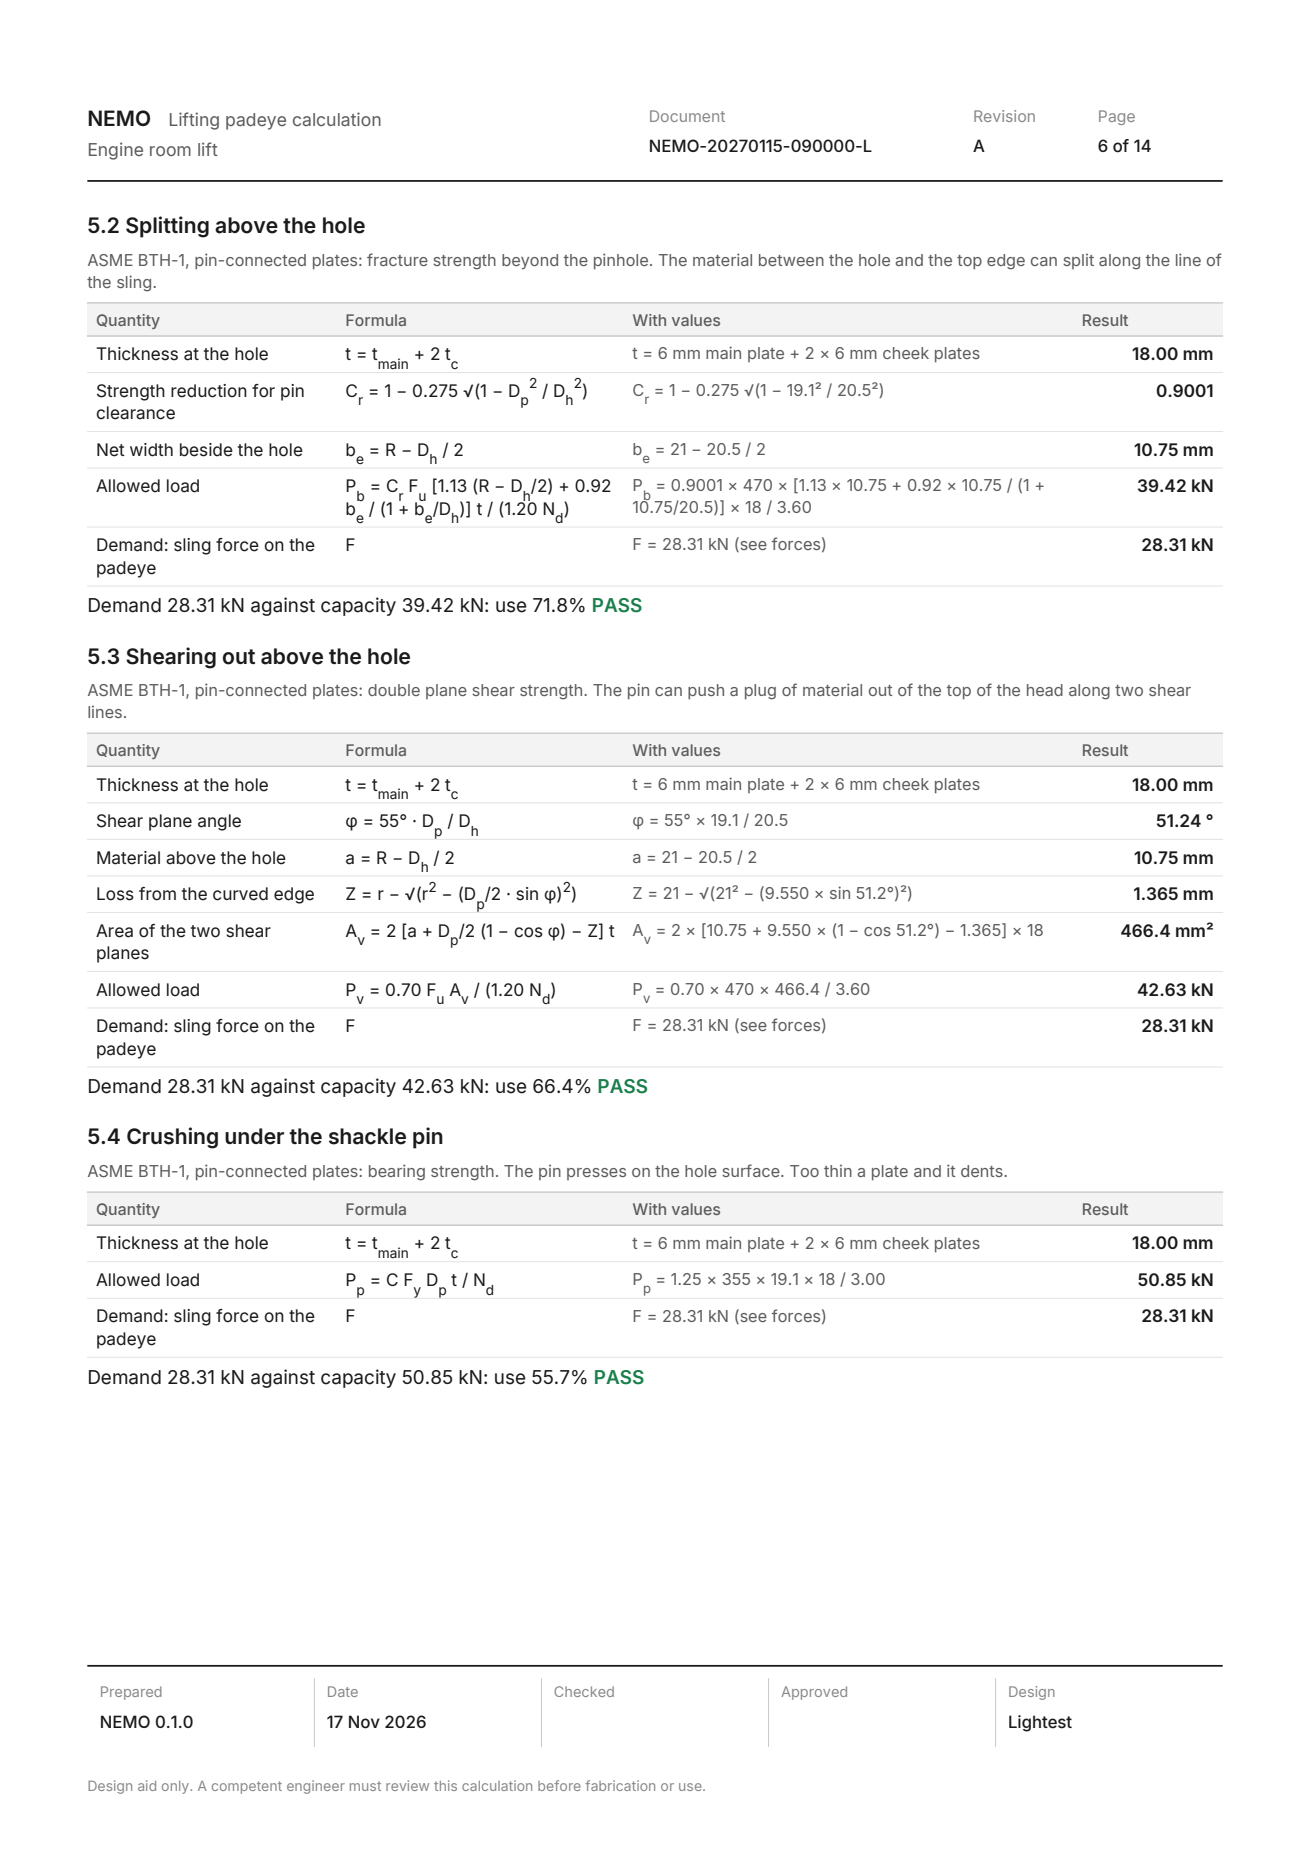
\includegraphics[width=\textwidth]{images/padeye-report-calc.png}
\caption{Check working}
\end{subfigure}
\caption{Pages from the calculation package of the lightest padeye}
\label{fig:padeye-report}
\end{figure}

\begin{figure}[H]
\centering
\begin{subfigure}{0.24\textwidth}
\centering
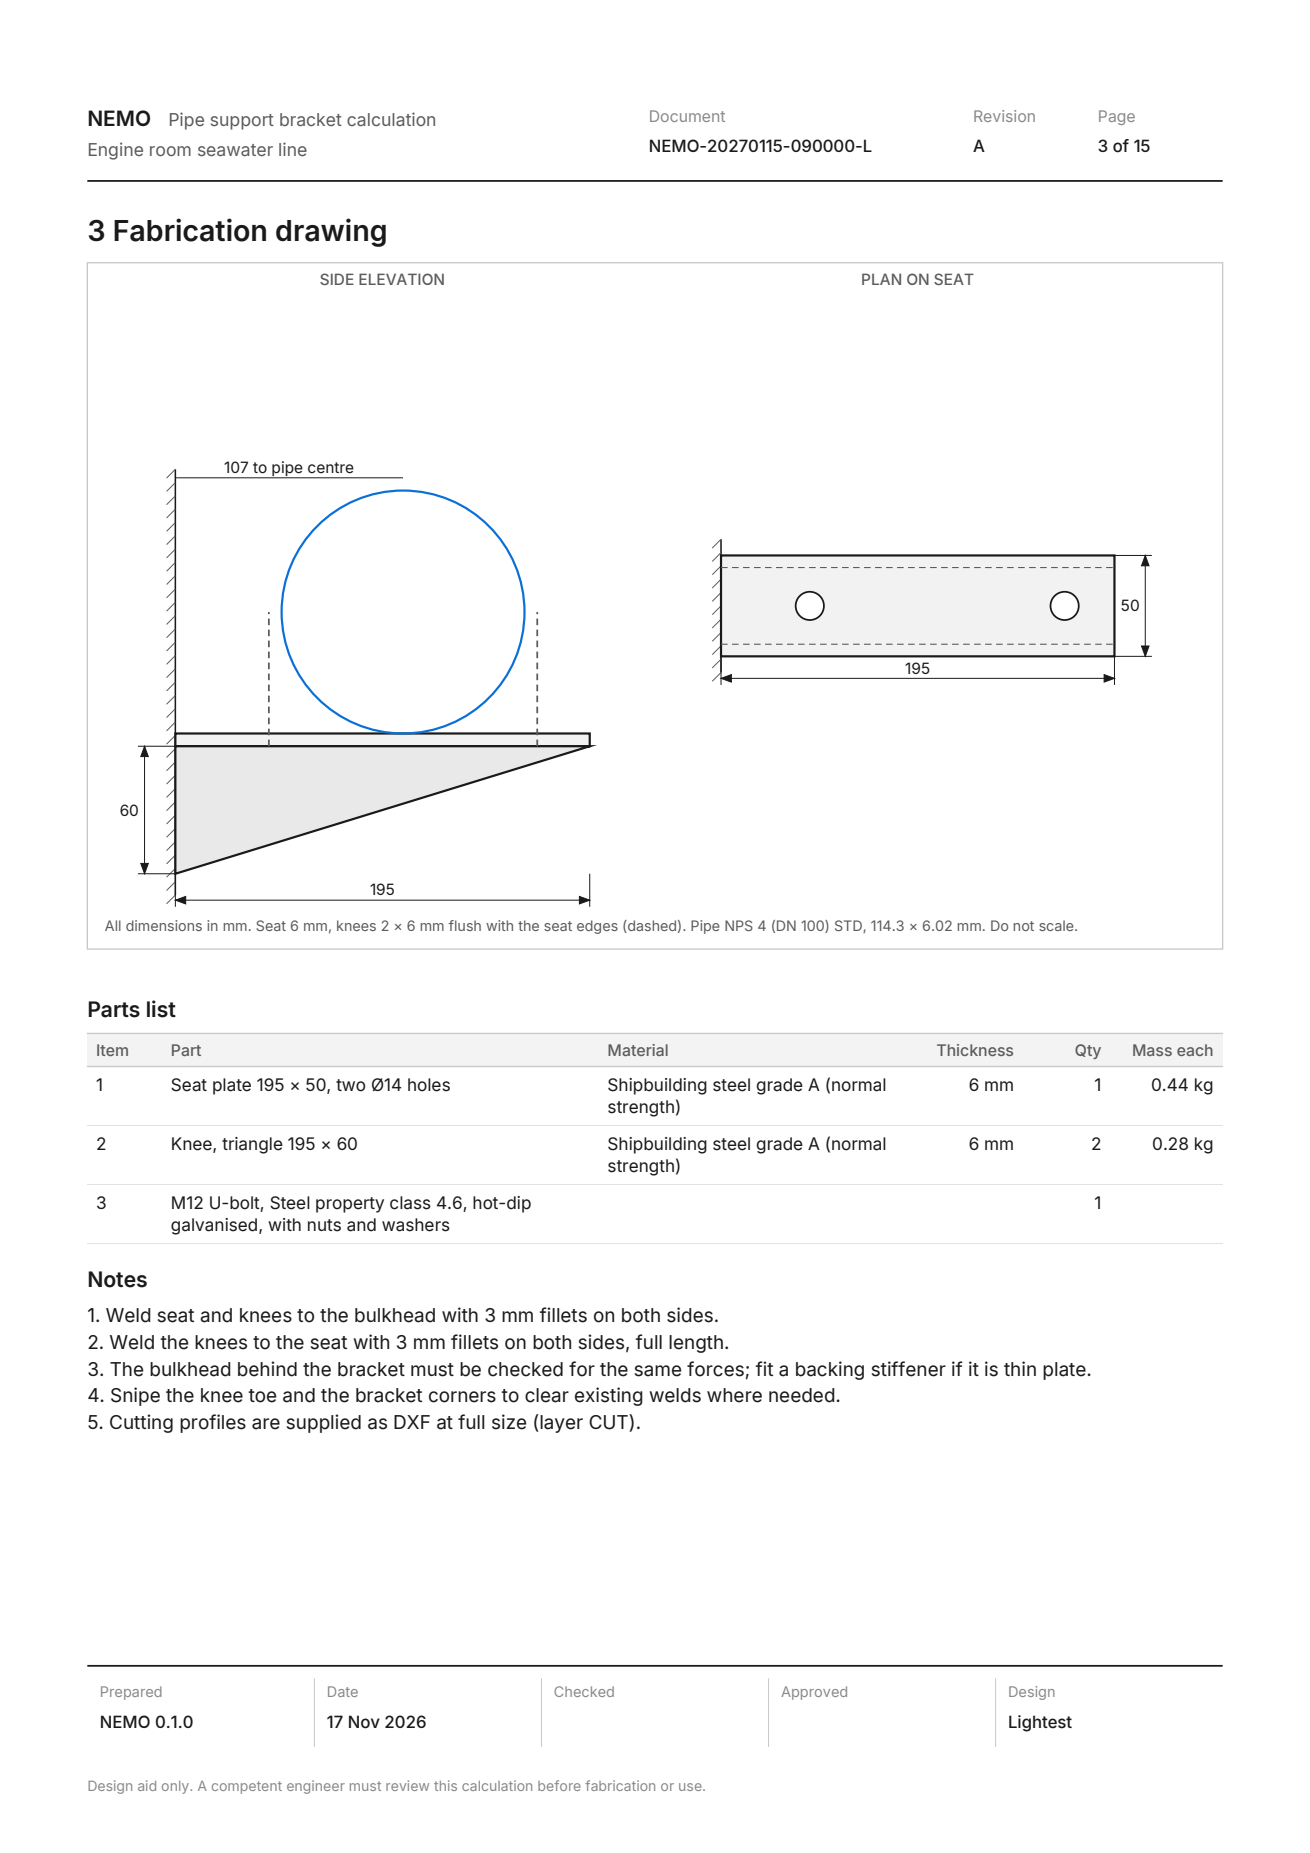
\includegraphics[width=\textwidth]{images/bracket-report-drawing.png}
\caption{Bracket drawing}
\end{subfigure}
\hfill
\begin{subfigure}{0.24\textwidth}
\centering
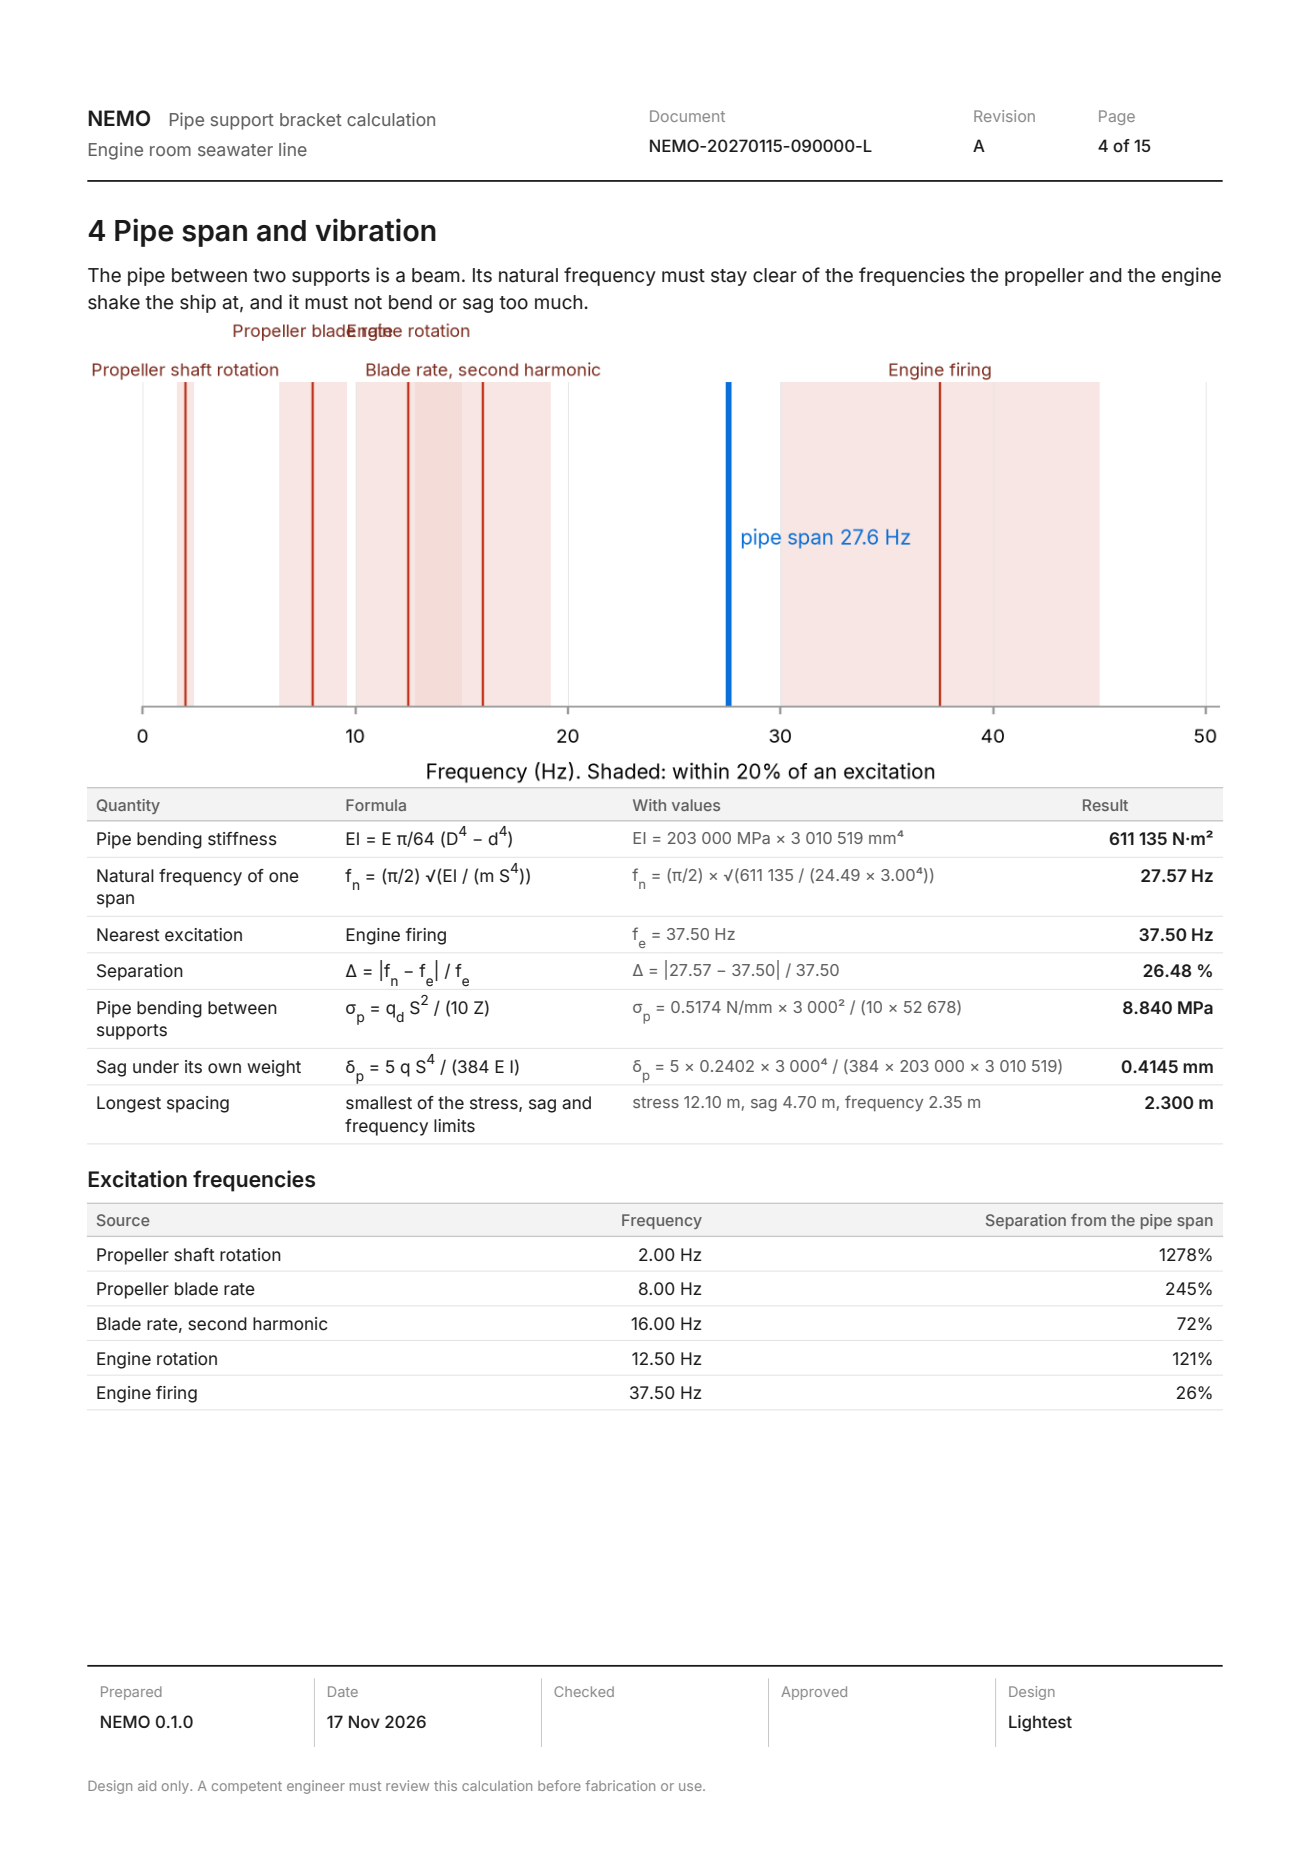
\includegraphics[width=\textwidth]{images/bracket-report-span.png}
\caption{Pipe span}
\end{subfigure}
\hfill
\begin{subfigure}{0.24\textwidth}
\centering
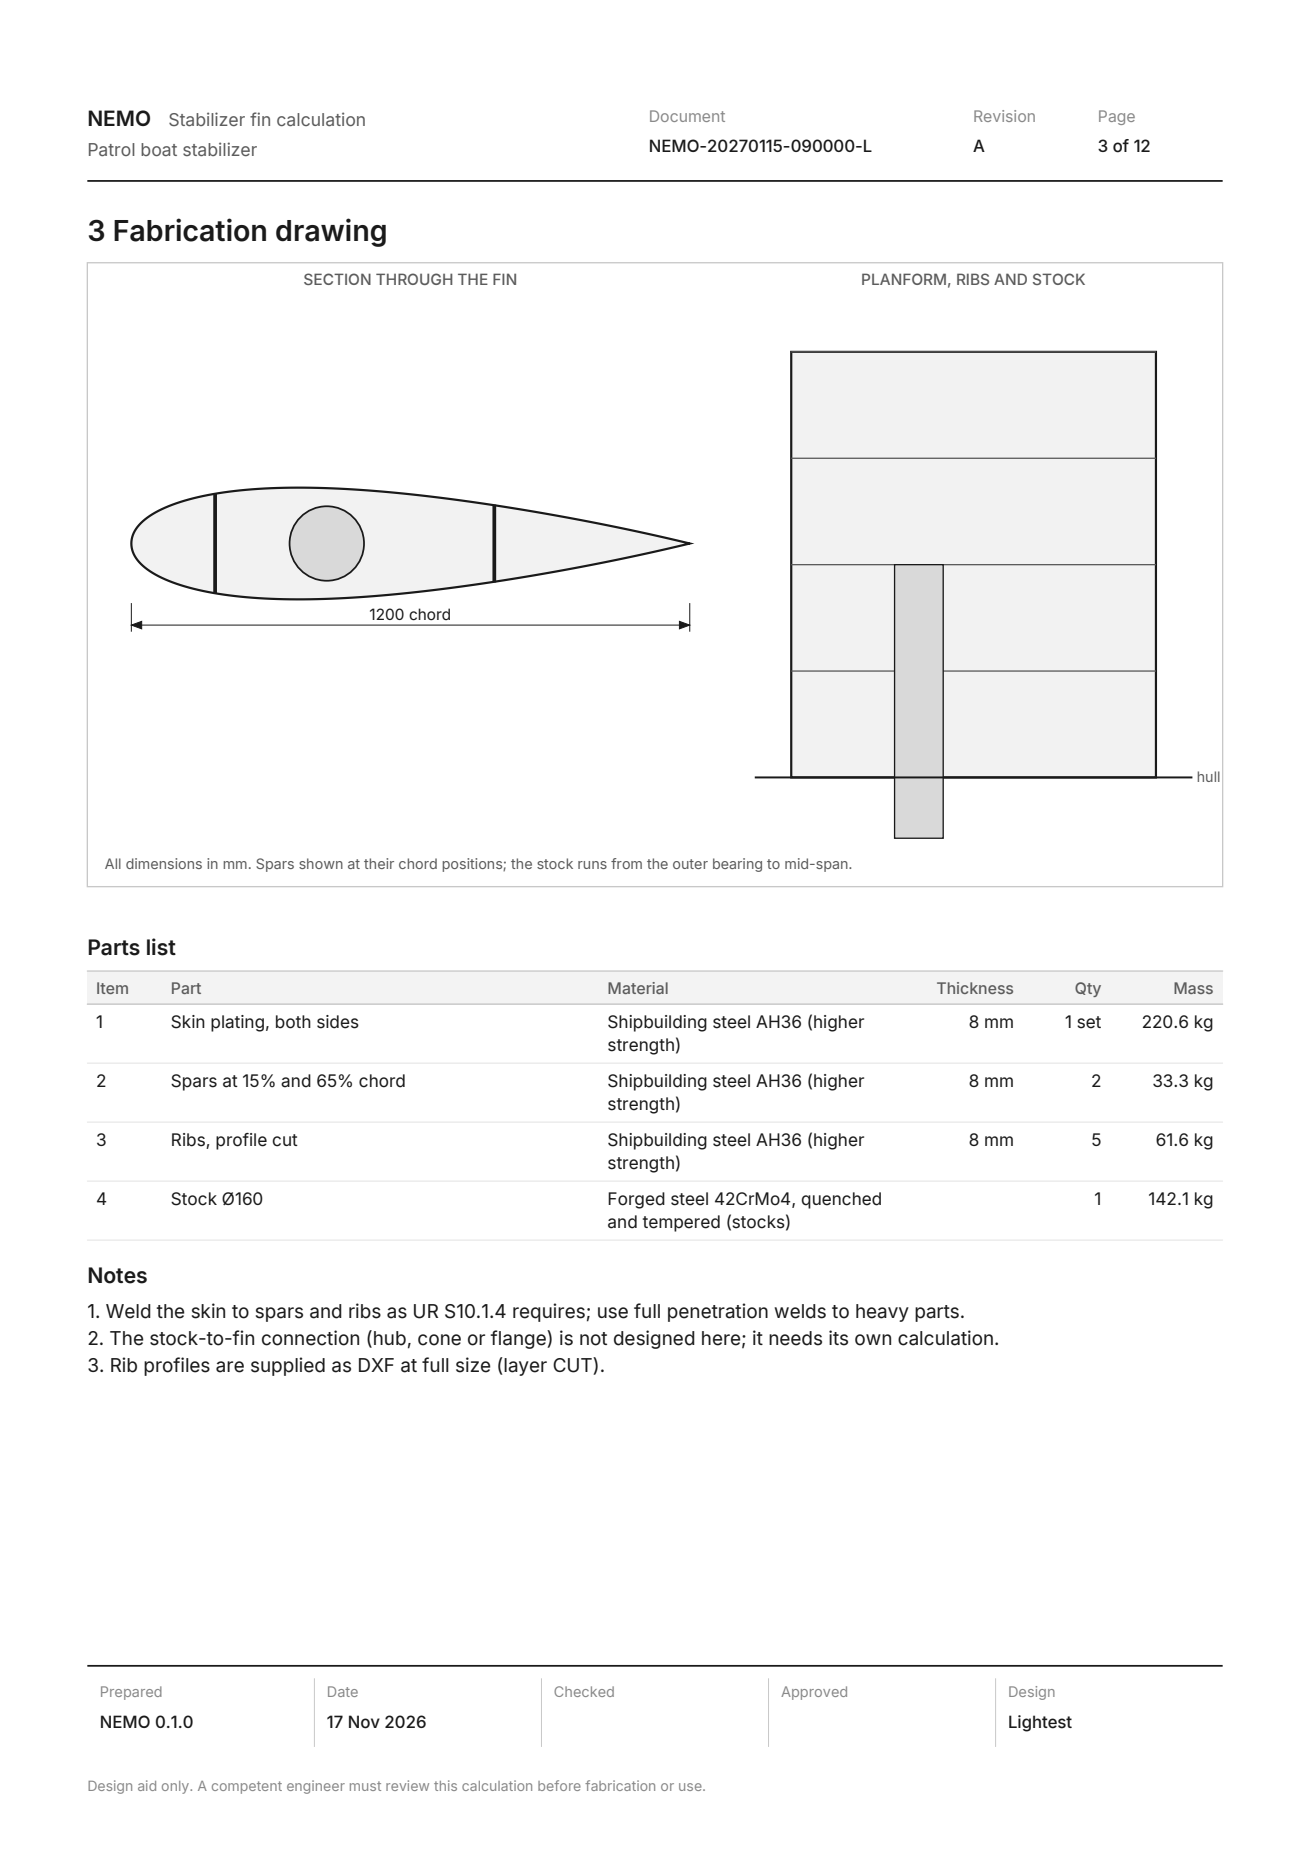
\includegraphics[width=\textwidth]{images/fin-report-drawing.png}
\caption{Fin drawing}
\end{subfigure}
\hfill
\begin{subfigure}{0.24\textwidth}
\centering
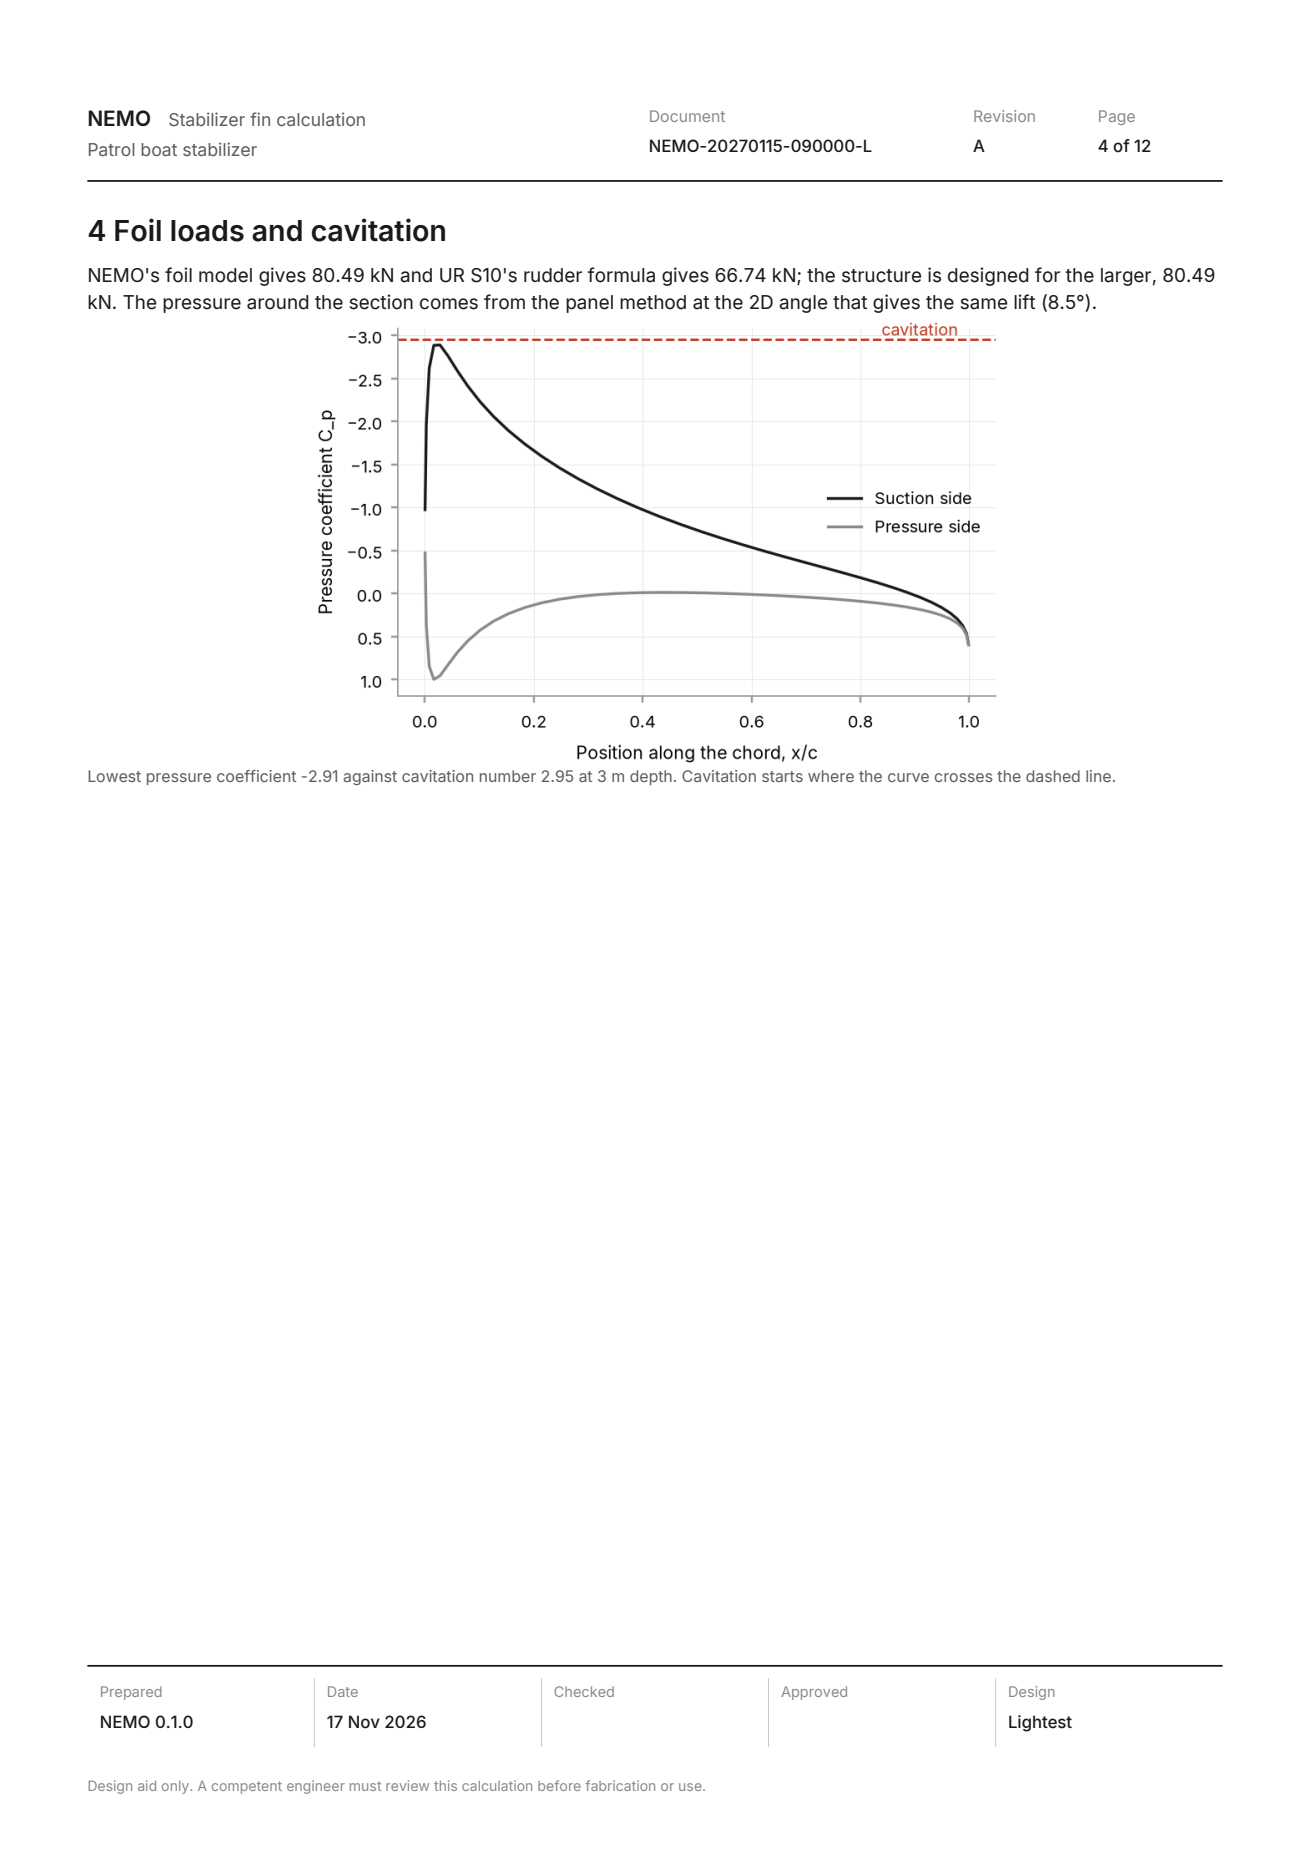
\includegraphics[width=\textwidth]{images/fin-report-foil.png}
\caption{Foil loads}
\end{subfigure}
\caption{Pages from the bracket and fin calculation packages}
\label{fig:other-reports}
\end{figure}

Figures~\ref{fig:app-results} to~\ref{fig:app-record} show the results
screens. The padeye results show the three designs side by side, the
dimensions of the selected one and its 3D model with the shackle and sling in
place. Selecting a check opens its working. The fin results show the stress in
the stock on the 3D model. The engineering record of the bracket lists the
steps of the run with their numbers, drawn from the engineering log.

\begin{figure}[H]
\centering
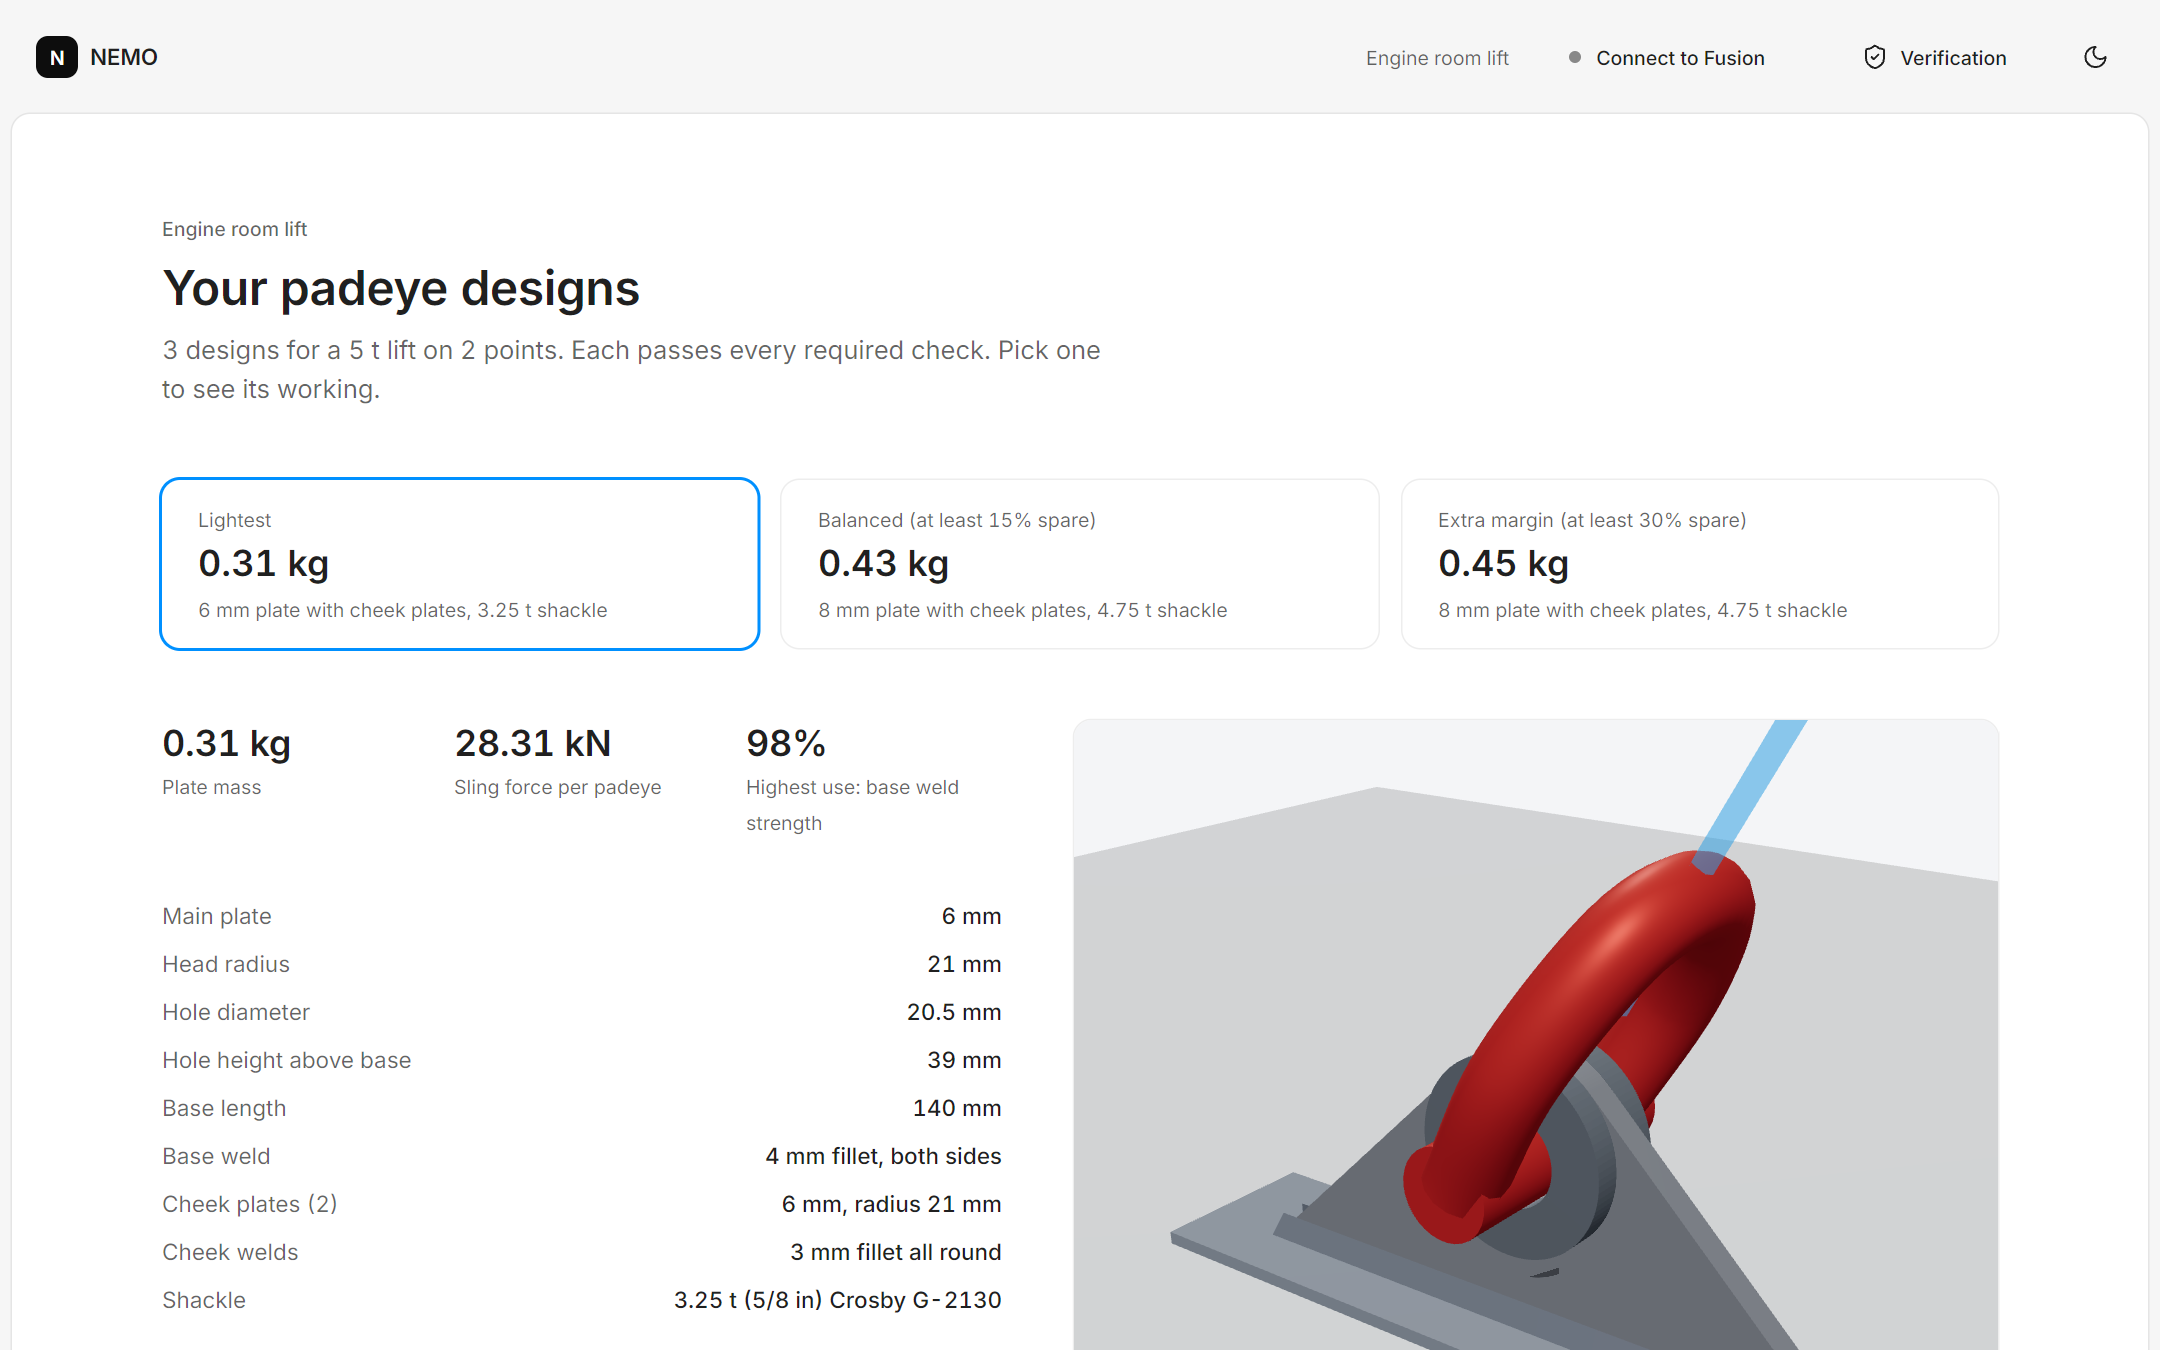
\includegraphics[width=0.85\textwidth]{images/app-padeye-results.png}
\caption{Padeye results, with the lightest of the three designs selected}
\label{fig:app-results}
\end{figure}

\begin{figure}[H]
\centering
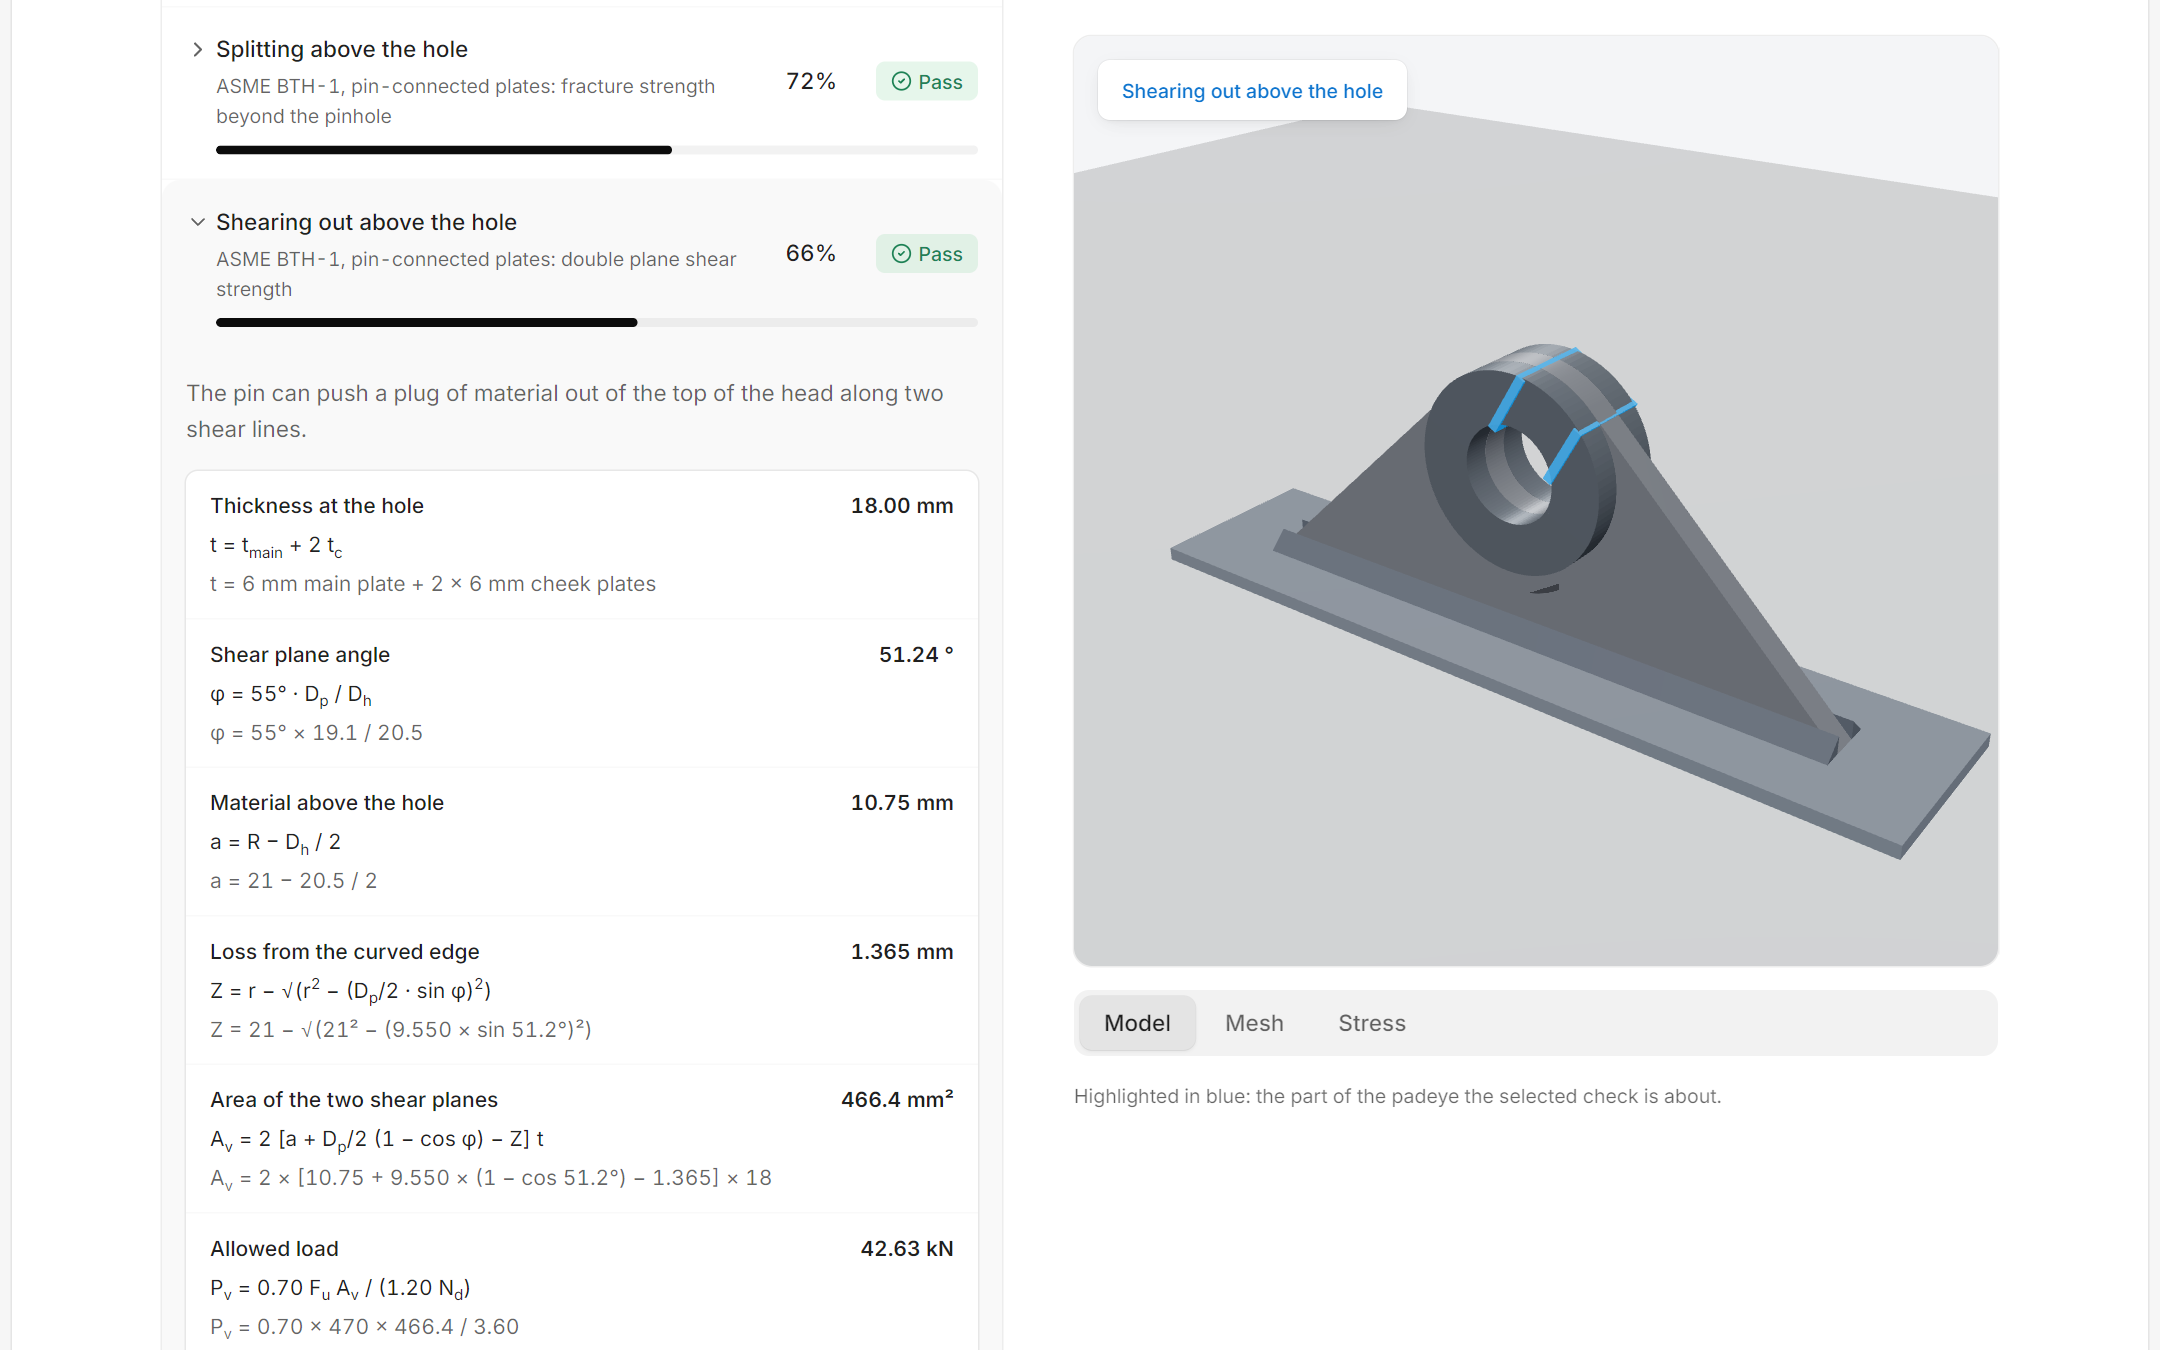
\includegraphics[width=0.85\textwidth]{images/app-padeye-check-working.png}
\caption{Working of a padeye check, as shown in the application}
\label{fig:app-check-working}
\end{figure}

\begin{figure}[H]
\centering
\begin{subfigure}{0.49\textwidth}
\centering
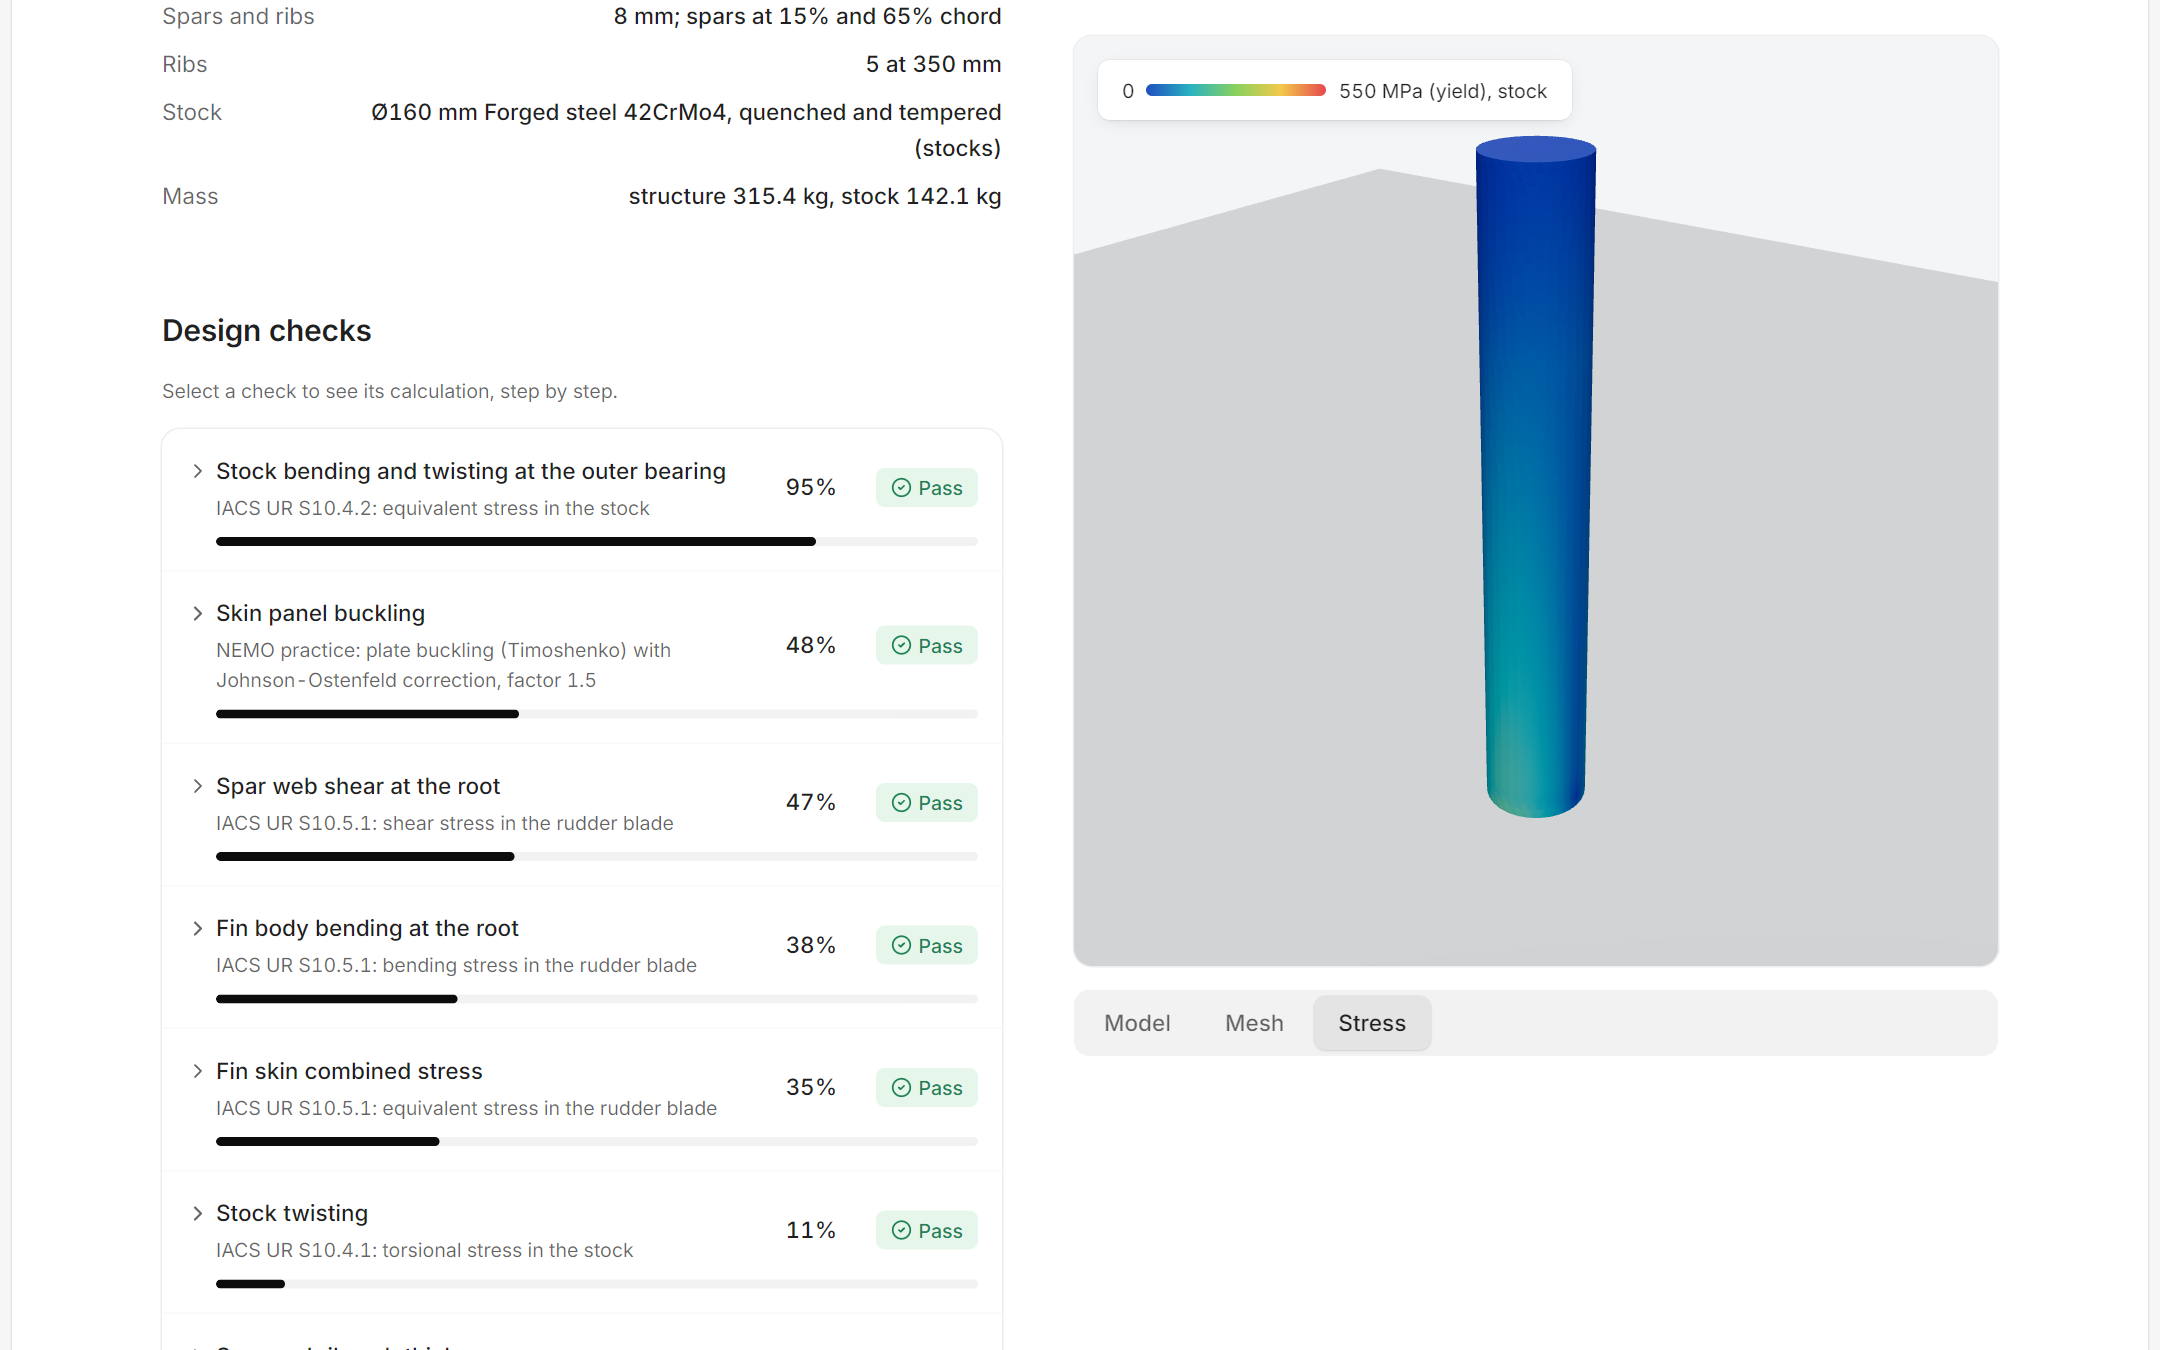
\includegraphics[width=\textwidth]{images/app-fin-results-stress.png}
\caption{Fin stock stress}
\end{subfigure}
\hfill
\begin{subfigure}{0.49\textwidth}
\centering
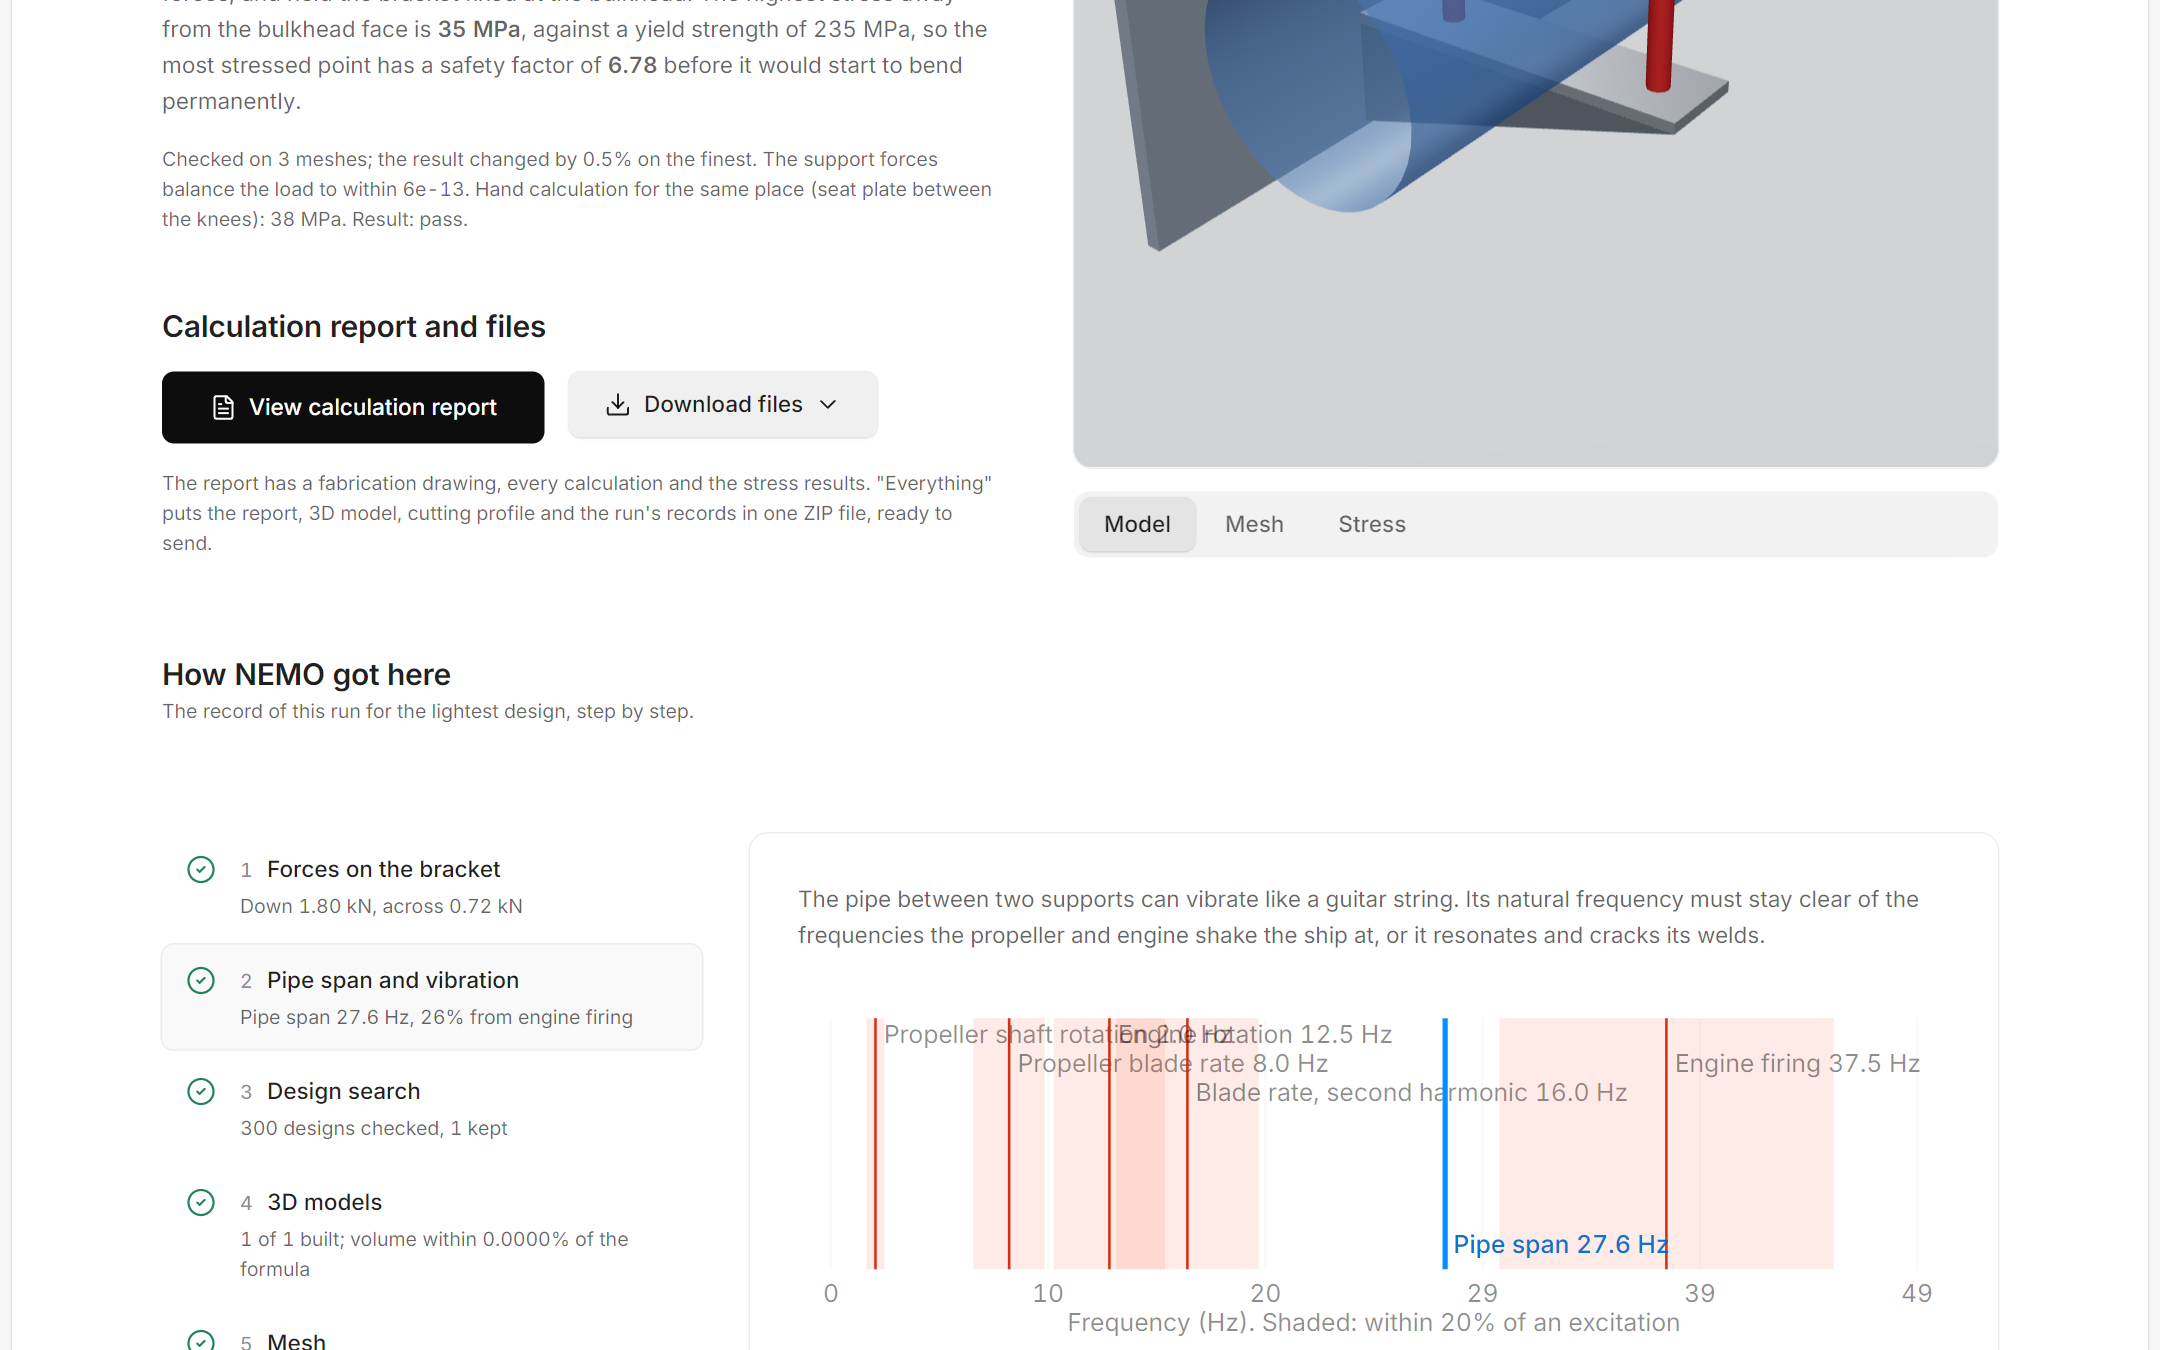
\includegraphics[width=\textwidth]{images/app-bracket-record.png}
\caption{Bracket engineering record}
\end{subfigure}
\caption{Fin and bracket results screens}
\label{fig:app-record}
\end{figure}

\section{Run times}
\label{sec:run-times}

Table~\ref{tab:run-times} gives the run times on the development computer,
running Windows. A run includes the search for all three targets, the CAD, the
three finite element solves for each design and the PDF packages.

\begin{table}[H]
\centering
\caption{Run times of the case studies}
\label{tab:run-times}
\small
\begin{tabular}{lrrrr}
\toprule
\textbf{Run} & \textbf{Designs tried} & \textbf{Kept} & \textbf{Largest model, unknowns} & \textbf{Time (s)}\\
\midrule
Padeye & 19,389 & 3 & 209,763 & 138.2\\
Bracket & 300 & 1 & 97,380 & 29.8\\
Fin & 3,780 & 3 & 75,831 & 79.9\\
Verification suite & & & 96,000 & 27.9\\
\bottomrule
\end{tabular}
\end{table}

Most of the padeye time is in the finite element solves. The three meshes of
the lightest design took 44~s together, and the finest mesh, with 209,763
unknowns, took 26.9~s. The search itself, 19,389 check evaluations, takes
less time than the analysis of one design. The live run screen shows progress
throughout, so the user can see which step is running and what it has found.

\section{Comparison with the first phase}
\label{sec:comparison}

Table~\ref{tab:comparison} compares the two phases against the requirements
of Table~\ref{tab:requirements}.

\begin{table}[H]
\centering
\caption{\NEMO{}~1 and \NEMO{}~2 compared}
\label{tab:comparison}
\small
\begin{tabularx}{\textwidth}{>{\raggedright\arraybackslash}p{0.2\textwidth}>{\raggedright\arraybackslash}X>{\raggedright\arraybackslash}X}
\toprule
\textbf{Aspect} & \textbf{\NEMO{}~1} & \textbf{\NEMO{}~2}\\
\midrule
Parts & Aluminium bracket, S275 padeye, aluminium fin & Steel padeye, pipe support bracket with pipe span, fin internal structure and stock\\
Design basis & Screening equations, some with unsourced factors & ASME BTH-1, AISC 360-16 and IACS UR S10 through replaceable rule sets; practice checks labelled\\
Fin load & Assumed & Whicker-Fehlner and UR S10, larger used; panel method for pressure and cavitation\\
Optimiser & Latin hypercube and Nelder-Mead on continuous variables & Stock plate enumeration, bounded Nelder-Mead, rounding, three targets\\
Stress analysis & Fusion Simulation, set up by hand; two bracket studies rejected & Built-in, three meshes per design, force balance and convergence checked automatically\\
Verification & None recorded & Six benchmarks with 24 compared quantities, and 153 automated tests\\
Traceability & Result files & Working for every check, engineering log, every design tried, checksums\\
Use & Python, virtual environment and Fusion needed & Installer and browser application; Fusion optional\\
Fusion link & File bridge that rebuilt stale requests & HTTP polling with expiring jobs; parametric model and re-check of edits\\
\bottomrule
\end{tabularx}
\end{table}

\section{Answers to the research questions}
\label{sec:research-answers}

\textbf{RQ1. Can one tool cover three structurally different marine details
while keeping every check traceable to a named rule or a stated practice?}
Yes, for the three parts built. The common check record, the rule-set
interface and the shared sizing and analysis pipeline served a pin-loaded
plate, a cantilever bracket with a vibration problem and a hydrodynamic foil
on a stock. Every check in Tables~\ref{tab:padeye-checks},
\ref{tab:bracket-checks-result} and~\ref{tab:fin-checks-result} names its
source, and the practice checks are labelled. The parts differ enough that
each needed its own load model and its own finite element set-up, so a new
part is still a substantial piece of work.

\textbf{RQ2. How closely do the built-in stress solver, geometry kernel and
foil solver agree with closed-form and published reference results?} The
geometry agrees exactly. The stress solver agrees within 0.8\% for
deflection, 2.6\% for beam stress, 0.9\% for a stress concentration and
0.13\% for the stock. The foil solver agrees within 0.05\% for the circle and
1.1\% to 1.7\% for the lift slope estimate. Force balance closed to
$10^{-11}$ or better on every model. These results show that the solvers are
implemented correctly. They do not validate the idealisations of the models,
such as the fixed supports or the cosine pin pressure.

\textbf{RQ3. What governs each part in practice, and what does that imply for
how such details are designed?} For the padeye, the base weld and the shackle
rating govern at moderate loads, and splitting above the hole at large loads.
Catalogue steps in the shackle drive the mass more than the plate dimensions.
For the bracket, minimum sizes govern the steel and pipe vibration governs the
spacing. Its strength checks reach only 25\%, while the span frequency limits
spacing to 2.3~m and the pass or fail result is not monotonic in spacing.
For the fin, the stock governs through the rule limit on combined stress, the
plating sits at rule minimums, the foil load exceeds the rule load by 21\%, and
cavitation limits the largest angle above about 18~knots. The common
implication is that a design method for these details must include the minimum
sizes, the catalogue and stock steps, the span and the hydrodynamics. A method
that only minimises mass under strength checks would miss what decides the
design in each case.

\textbf{RQ4. Can a non-programmer run the full workflow, from job description
to calculation package, unaided?} The tool removes the technical barriers. It
installs from one file, the forms ask for the job in plain words, and the run,
results and package need no code. Whether a non-programmer can complete the
workflow unaided has not been tested with users. A formal usability study is
needed to answer this question, and it is listed in
Section~\ref{sec:future-work}.

\section{Limitations}
\label{sec:limitations}

The results above have the following limits, which a user of the tool should
know.

\begin{itemize}
    \item \textbf{No physical tests.} All verification is against hand
    calculations, theory and published coefficients. No padeye, bracket or fin
    designed by the tool has been built or load tested.
    \item \textbf{BTH-1 reading not checked against a worked example.} The code
    matches the engineering manual, but the manual has not been compared with
    a published BTH-1 padeye example.
    \item \textbf{Ship-motion accelerations are inputs.} The bracket loads are
    only as good as the accelerations the user enters. The tool does not
    compute them from a classification society method.
    \item \textbf{Simplified span model.} The pipe span is treated as a simply
    supported beam on rigid supports. Flexible supports, bends, valves and
    fluid flow change the frequency and are not modelled.
    \item \textbf{Quasi-static fin loads.} The fin is checked under the steady
    load at its largest angle. Dynamic loads from fin motion, waves, slamming
    and the control system are not included. The panel method is inviscid and
    gives cavitation onset only.
    \item \textbf{Rudder rules applied to a fin.} UR S10 is written for
    rudders. It is the nearest published basis, but its use does not amount to
    class approval of a fin.
    \item \textbf{Finite element scope.} The finite element models are linear
    elastic, do not include the welds, and model the fin stock alone. They
    confirm the hand checks in the regions they cover.
    \item \textbf{Fusion connector untested in Fusion.} The add-in has not yet
    been run in a live Fusion session, and no Fusion stress cross-check has
    been recorded.
    \item \textbf{No usability study.} Ease of use has been designed for but
    not measured.
\end{itemize}
